%% Chapter 1 — Substrate.
%%
%% Premise: a large language model is a fixed set of numbers left behind by training; one run
%% of it scores which fragment of text plausibly comes next, and running it repeatedly is what
%% produces an answer.
%%
%% Rebuilt 2026-08-20 against the instructor's per-slide review. Four changes drive the shape:
%%   1. The slide order follows the pipeline diagram left to right, because the diagram promises
%%      a path and the previous version went back and forth across it.
%%   2. One running example for the whole chapter: the stirrups sentence.
%%   3. A new slide between fitting and scoring, carrying the step the chapter was missing —
%%      what training minimises is defined in terms of a probability, so the output has to be a
%%      distribution. That is the bridge from "everything is deterministic" to "the same prompt
%%      gives different answers".
%%   4. Greedy selection failing now comes BEFORE sampling is introduced, so the sampler has a
%%      reason rather than being asserted.
\documentclass[aspectratio=169,11pt]{beamer}
\usetheme{UHTraining}
%% Shared preamble for the course decks.
\usepackage{uhcite}
\usepackage{uhslot}
\usepackage{amsmath}
\usetikzlibrary{arrows.meta,positioning}

%% --- the four kinds of number ------------------------------------------------
%% A review found parameters, token IDs, logits and probabilities were all appearing as
%% bare numbers with nothing telling them apart. Each now has one colour, used identically
%% in the slides, the figures and the animations. Colour is a redundant cue: every coloured
%% number carries its word too, so nothing depends on hue alone.
\newcommand{\tokid}[1]{\textcolor{uhslate}{\textbf{#1}}}   % a label, no magnitude
\newcommand{\param}[1]{\textcolor{uhocher}{\textbf{#1}}}   % the fitted numbers
\newcommand{\logit}[1]{\textcolor{uhteal}{\textbf{#1}}}    % raw scores out of the network
\newcommand{\prob}[1]{\textcolor{uhred}{\textbf{#1}}}      % probabilities
%% Defined terms are bold and black. Colour is reserved for number kinds, so that a colour
%% on a slide always answers the same question: what sort of number is this?
\newcommand{\kw}[1]{\textbf{#1}}
%% Inside an equation the same colours apply without \textbf, which is text-mode and breaks
%% on a subscript. Colour only; maths keeps its own italic.
\newcommand{\mlogit}[1]{\textcolor{uhteal}{#1}}
\newcommand{\mprob}[1]{\textcolor{uhred}{#1}}

%% --- a figure that an animation replaces in the PowerPoint version ------------
\newcommand{\animatable}[2]{%
  \vspace{-0.5em}{\scriptsize\color{uhocher}\textbf{animation #1} replaces this figure --- #2}\par}

%% --- diagram styles ----------------------------------------------------------
\tikzset{
  uhbox/.style   ={draw=uhslate!70, fill=uhslate!7,  rounded corners=1pt, align=center,
                   font=\scriptsize, inner sep=3pt, minimum height=8mm, text width=19mm},
  uhwide/.style  ={uhbox, text width=26mm},
  uhhi/.style    ={uhbox, draw=uhred, fill=uhred!8, thick},
  uhamber/.style ={uhbox, draw=uhocher, fill=uhocher!12, thick},
  uhghost/.style ={uhbox, draw=uhslate!45, fill=none, dashed},
  uhar/.style    ={-{Latex[length=1.8mm]}, draw=uhslate!80, thick},
  uhardot/.style ={-{Latex[length=1.8mm]}, draw=uhslate!55, thick, dashed},
}

% Generated from references.md by gen-sources-tex.mjs. Do not edit by hand.
\uhdefsource{vaswani2017}{V}{Vaswani, A., Shazeer, N., Parmar, N., Uszkoreit, J., Jones, L., Gomez, A. N., Kaiser, L. \& Polosukhin, I., 2017. \emph{Attention Is All You Need}, arXiv:1706.03762.}{}
\uhdefsource{anthropic-code-exec}{V}{Anthropic, 2026. \emph{Code execution tool, platform.claude.com --- vendor documentation, fetched 2026-08-20}.}{}
\uhdefsource{kaplan2020}{V}{Kaplan, J., McCandlish, S., Henighan, T., et al., 2020. \emph{preprint}, arXiv:2001.08361.}{}
\uhdefsource{hoffmann2022}{V}{Hoffmann, J., Borgeaud, S., Mensch, A., et al., 2022. \emph{preprint --- venue unconfirmed}, arXiv:2203.15556.}{}
\uhdefsource{fedus2021}{V}{Fedus, W., Zoph, B. \& Shazeer, N., 2021. \emph{arXiv preprint; version of record JMLR 23(120):1--39, 2022}, arXiv:2101.03961.}{}
\uhdefsource{lepikhin2020}{V}{Lepikhin, D., Lee, H., Xu, Y., et al., 2020. \emph{arXiv preprint; ICLR 2021}, arXiv:2006.16668.}{}
\uhdefsource{clark2022}{V}{Clark, A., de las Casas, D., Guy, A., et al., 2022. \emph{ICML 2022, pp. 4057--4086}, arXiv:2202.01169.}{}
\uhdefsource{stiennon2020}{V}{Stiennon, N., Ouyang, L., Wu, J., et al., 2020. \emph{preprint --- venue unconfirmed}, arXiv:2009.01325.}{}
\uhdefsource{ouyang2022}{V}{Ouyang, L., Wu, J., Jiang, X., et al., 2022. \emph{NeurIPS 2022}, arXiv:2203.02155.}{}
\uhdefsource{bai2022hh}{V}{Bai, Y., Jones, A., Ndousse, K., et al., 2022. \emph{preprint}, arXiv:2204.05862.}{}
\uhdefsource{bai2022cai}{V}{Bai, Y., Kadavath, S., Kundu, S., et al., 2022. \emph{preprint}, arXiv:2212.08073.}{}
\uhdefsource{rafailov2023}{V}{Rafailov, R., Sharma, A., Mitchell, E., Ermon, S., Manning, C. D. \& Finn, C., 2023. \emph{NeurIPS 2023}, arXiv:2305.18290.}{}
\uhdefsource{ye2024}{V}{Ye, Q., Axmed, M., Pryzant, R. \& Khani, F., 2024. \emph{Findings of the ACL 2024}, arXiv:2311.05661.}{}
\uhdefsource{li2023emotion}{V}{Li, C., Wang, J., Zhang, Y., et al., 2023. \emph{technical report, not peer reviewed}, arXiv:2307.11760.}{}
\uhdefsource{vaugrante2024}{V}{Vaugrante, L., Niepert, M. \& Hagendorff, T., 2024. \emph{preprint --- venue unconfirmed}, arXiv:2409.20303.}{}
\uhdefsource{yang2023}{V}{Yang et al., 2023. \emph{Google DeepMind; arXiv preprint (ICLR 2024 per the arXiv comment)}, arXiv:2309.03409.}{}
\uhdefsource{wei2022}{V}{Wei, J., Wang, X., Schuurmans, D., Bosma, M., Ichter, B., Xia, F., Chi, E., Le, Q. \& Zhou, D., 2022. \emph{Chain-of-Thought Prompting Elicits Reasoning in Large Language Models}, arXiv:2201.11903.}{}
\uhdefsource{anthropic-prompting}{V}{Anthropic, 2026. \emph{Prompting best practices, platform.claude.com --- vendor documentation, fetched 2026-08-19}.}{}
\uhdefsource{anthropic-models}{V}{Anthropic, 2026. \emph{Models overview, platform.claude.com --- vendor documentation, fetched 2026-08-20}.}{}
\uhdefsource{anthropic-thinking}{V}{Anthropic, 2026. \emph{Steering thinking, platform.claude.com --- vendor documentation, fetched 2026-08-20}.}{}
\uhdefsource{erratum2026}{V}{Reader comment (unattributed), 2026. \emph{Comment thread on the Pope lecture transcript gist --- reader correction, not a primary result}.}{testimony}
\uhdefsource{zheng2024}{V}{Zheng, M., Pei, J., Logeswaran, L., Lee, M. \& Jurgens, D., 2024. \emph{Findings of the ACL: EMNLP 2024, pp. 15126--15154}, DOI 10.18653/v1/2024.findings-emnlp.888.}{}
\uhdefsource{liu2024}{V}{Liu, N. F., Lin, K., Hewitt, J., Paranjape, A., Bevilacqua, M., Petroni, F. \& Liang, P., 2024. \emph{Transactions of the ACL 12, pp. 157--173}, DOI 10.1162/tacl\_a\_00638.}{}
\uhdefsource{velickovic2025}{V}{Veličković, P., Perivolaropoulos, C., Barbero, F. \& Pascanu, R., 2025. \emph{ICML 2025, PMLR 267, pp. 61190--61211}, arXiv:2410.01104.}{}
\uhdefsource{kamradt2023}{V}{Kamradt, G., 2023. \emph{Needle in a Haystack --- software implementation, not a peer-reviewed result}, github.com/gkamradt/needle-in-a-haystack.}{}
\uhdefsource{chroma2025}{V}{Hong, K., Troynikov, A. \& Huber, J., 2025. \emph{Chroma technical report --- COI, see below}, trychroma.com/research/context-rot.}{coi}
\uhdefsource{liang2023}{V}{Liang, W., Yuksekgonul, M., Mao, Y., Wu, E. \& Zou, J., 2023. \emph{Patterns 4(7):100779}, DOI 10.1016/j.patter.2023.100779.}{}
\uhdefsource{dathathri2024}{V}{Dathathri, S., See, A., Ghaisas, S., et al., 2024. \emph{Nature 634(8035), pp. 818--823}, DOI 10.1038/s41586-024-08025-4.}{}
\uhdefsource{bricken2023}{V}{Bricken, T., Templeton, A., Batson, J., et al., 2023. \emph{Anthropic, Transformer Circuits Thread --- COI, lab publishing on its own models}, transformer-circuits.pub.}{coi}
\uhdefsource{templeton2024}{V}{Templeton, A., Conerly, T., Marcus, J., et al., 2024. \emph{Anthropic, Transformer Circuits Thread --- COI, lab publishing on its own models}, arXiv:2605.29358.}{coi}
\uhdefsource{ameisen2025}{V}{Ameisen, E., Lindsey, J., Pearce, A., et al., 2025. \emph{Anthropic, Transformer Circuits Thread --- COI, lab publishing on its own models}, transformer-circuits.pub.}{coi}
\uhdefsource{lindsey2025}{V}{Lindsey, J., Gurnee, W., Ameisen, E., et al., 2025. \emph{Anthropic, Transformer Circuits Thread --- COI, lab publishing on its own models}, transformer-circuits.pub.}{coi}
\uhdefsource{turpin2023}{V}{Turpin, M., Michael, J., Perez, E. \& Bowman, S. R., 2023. \emph{NeurIPS 2023}, arXiv:2305.04388.}{}
\uhdefsource{chen2025}{V}{Chen, Y., Benton, J., Radhakrishnan, A., et al., 2025. \emph{Anthropic --- COI, lab publishing on its own models}, arXiv:2505.05410.}{coi}
\uhdefsource{greshake2023}{V}{Greshake, K., Abdelnabi, S., Mishra, S., Endres, C., Holz, T. \& Fritz, M., 2023. \emph{AISec '23, pp. 79--90}, DOI 10.1145/3605764.3623985.}{}
\uhdefsource{owasp2026}{V}{OWASP GenAI Security Project, 2026. \emph{OWASP Top 10 for LLM Applications, 2026 edition}, LLM01:2026.}{}
\uhdefsource{cohen2025}{V}{Cohen, S., Bitton, R. \& Nassi, B., 2025. \emph{ACM CCS 2025, pp. 3975--3989}, DOI 10.1145/3719027.3765196.}{}
\uhdefsource{aisi2026}{V}{UK AI Security Institute, 2026. \emph{Incident report, aisi.gov.uk --- blog page read; technical report not read}, INC-2026-07-28-01.}{}
\uhdefsource{pope2026}{V}{Pope, R., 2026. \emph{Dwarkesh Podcast, blackboard lecture; transcript published as a public gist}.}{testimony,coi}
\uhdefsource{revnets}{V}{Gomez, A. N., Ren, M., Urtasun, R. \& Grosse, R. B., 2017. \emph{The Reversible Residual Network: Backpropagation Without Storing Activations}, arXiv:1707.04585.}{}
\uhdefsource{ornes2025}{V}{Ornes, S., 2025. \emph{PNAS 122(44) --- secondary account, not primary research}, DOI 10.1073/pnas.2528654122.}{}
\uhdefsource{smirnova2023}{V}{Smirnova, L., Caffo, B. S., Gracias, D. H., et al., 2023. \emph{Frontiers in Science 1}, DOI 10.3389/fsci.2023.1017235.}{}
\uhdefsource{schrimpf2021}{V}{Schrimpf, M., Blank, I. A., Tuckute, G., et al., 2021. \emph{PNAS 118(45):e2105646118}, DOI 10.1073/pnas.2105646118.}{}
\uhdefsource{goldstein2022}{V}{Goldstein, A., Zada, Z., Buchnik, E., et al., 2022. \emph{Nature Neuroscience 25(3):369--380}, DOI 10.1038/s41593-022-01026-4.}{}
\uhdefsource{antonello2024}{V}{Antonello, R. \& Huth, A., 2024. \emph{Neurobiology of Language 5(1):64--79}, DOI 10.1162/nol\_a\_00087.}{}
\uhdefsource{hadidi2026}{V}{Hadidi, N., Feghhi, E., Song, B. H., Blank, I. A. \& Kao, J. C., 2026. \emph{Nature Communications 17(1):5769}, DOI 10.1038/s41467-026-72253-7.}{}
\uhdefsource{fedorenko2024}{V}{Fedorenko, E., Piantadosi, S. T. \& Gibson, E. A. F., 2024. \emph{Nature 630(8017)}, DOI 10.1038/s41586-024-07522-w.}{}
\uhdefsource{diachek2020}{V}{Diachek, E., Blank, I., Siegelman, M., Affourtit, J. \& Fedorenko, E., 2020. \emph{Journal of Neuroscience 40(23):4536--4550}, DOI 10.1523/JNEUROSCI.2036-19.2020.}{}
\uhdefsource{cowan2001}{V}{Cowan, N., 2001. \emph{Behavioral and Brain Sciences 24(1):87--114, discussion 114--185}, DOI 10.1017/S0140525X01003922.}{}
\uhdefsource{claudecode-docs}{V}{Anthropic, 2026. \emph{Claude Code documentation, code.claude.com --- vendor documentation, version-dependent}.}{}
\uhdefsource{anthropic-support}{V}{Anthropic, 2026. \emph{Anthropic support centre, support.claude.com --- vendor documentation, version-dependent}.}{}
\uhdefsource{graphify}{V}{Graphify project, 2026. \emph{graphify 0.9.16, behaviour observed directly on this machine 2026-08-19}, version 0.9.16.}{}
\uhdefsource{mcp-spec}{V}{Model Context Protocol, 2025-06-18. \emph{modelcontextprotocol.io --- protocol specification}, version 2025-06-18.}{}
\uhdefsource{anthropic-pdf}{V}{Anthropic, 2026. \emph{PDF support, platform.claude.com --- vendor documentation, fetched 2026-08-20}.}{}


\courseflowreset
\courseflowstep{Substrate}{}
\courseflowstep{Formation}{}
\courseflowstep{Control}{}
\courseflowstep{Measure}{}
\courseflowstep{Failure}{}
\courseflowstep{Limits}{}
\courseflowcurrent{1}
\uhshorttitle{Chapter 1 --- Substrate}

\title{Chapter 1 --- Substrate}
\subtitle{What a language model is, and what one run of it computes}
\author{AI Training}
\institute{University of Houston}
\date{2026}

\graphicspath{{../../assets/figures/}}

\begin{document}

% ---------------------------------------------------------------- 1
\begin{frame}[plain]
  \titlepage
  \provenance{none}
\end{frame}
\note{Nothing in this chapter assumes the room has seen any of it before. Say that out loud.}

% ---------------------------------------------------------------- 2
\begin{frame}{The answer arrives a piece at a time}
  \slotF{a question typed, and the reply appearing left to right at natural speed}

  {\small The text you send is the \kw{prompt}. Every character counts, spaces and typos included,
   and it can carry images too. The reply comes back a piece at a time.}
  \provenance{observation}
\end{frame}
\note{%
Opens on the one thing every attendee has already seen, and plants the puzzle the chapter pays
off at the end: the same question, asked twice, gives two different answers. Do not explain it
here. Say it is odd, and that by the last slide it will be obvious.\\[0.3em]
Caveat worth saying: some interfaces buffer and show the reply whole. The pieces are still
produced one at a time; only the display differs.}

% ---------------------------------------------------------------- 3
\begin{frame}{Language models are one branch of AI}
  \begin{center}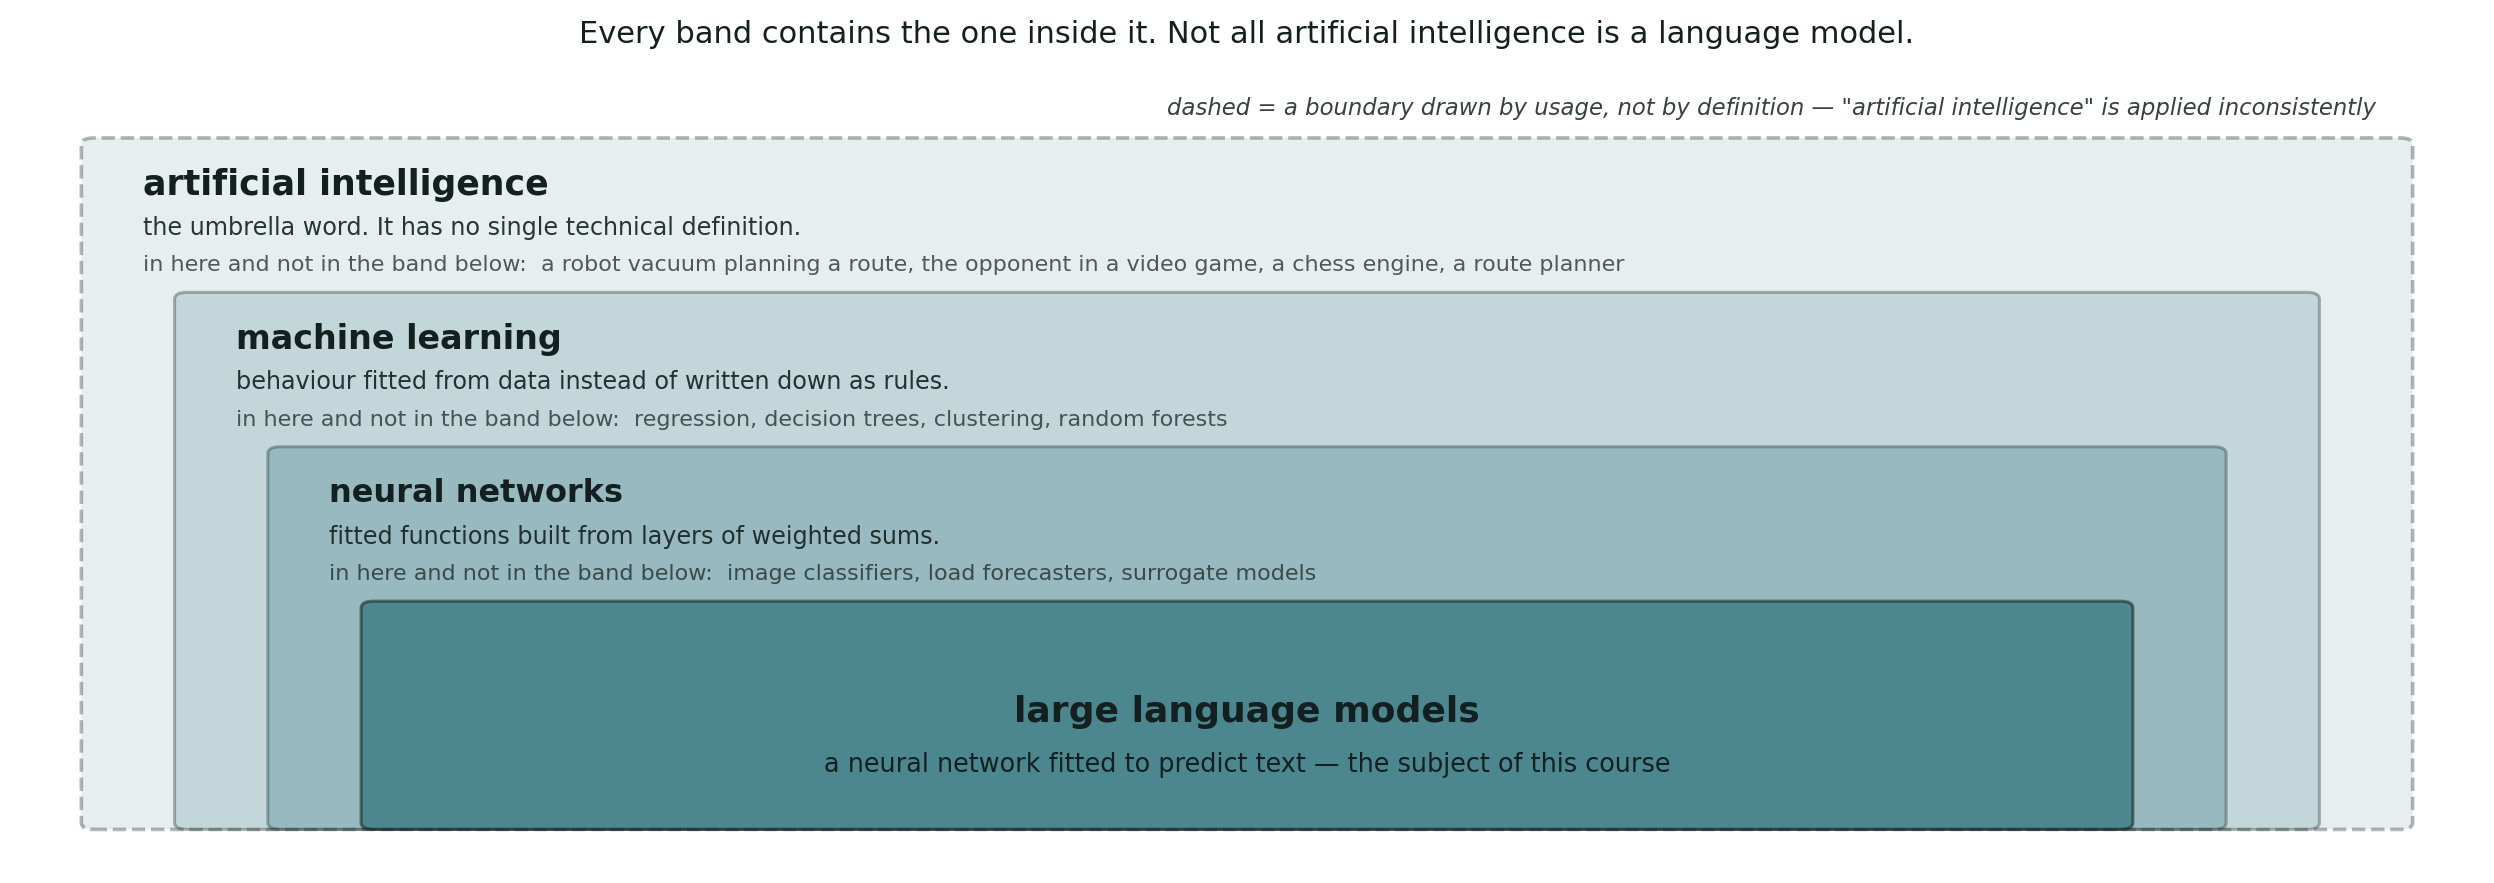
\includegraphics[height=39mm,width=\linewidth,keepaspectratio]{01-what-is-ai}\end{center}
  {\small A \kw{neural network} is a fitted function of layered weighted sums. A \kw{large
   language model} is one fitted to predict text.}
  \provenance{definition}
\end{frame}
\note{%
Answers "is all AI an LLM?" --- no --- and bounds every claim the course makes afterwards.\\[0.3em]
Concrete examples land this faster than the diagram does. A robot vacuum planning a route has AI.
The opponent in a video game has AI. A chess engine has AI. None of them is a language model, and
none of them shares any machinery with one.\\[0.3em]
The outer boundary is drawn dashed on purpose: artificial intelligence has no single technical
definition, and what sits under the label has changed several times. The inner three genuinely
nest --- a large language model IS a neural network, IS fitted from data.\\[0.3em]
One caveat if asked: not every language model is a neural network. Word-frequency models predate
them. Every model in this course is one.}

% ---------------------------------------------------------------- 4
\begin{frame}{Reliability follows how much was written}
  \begin{center}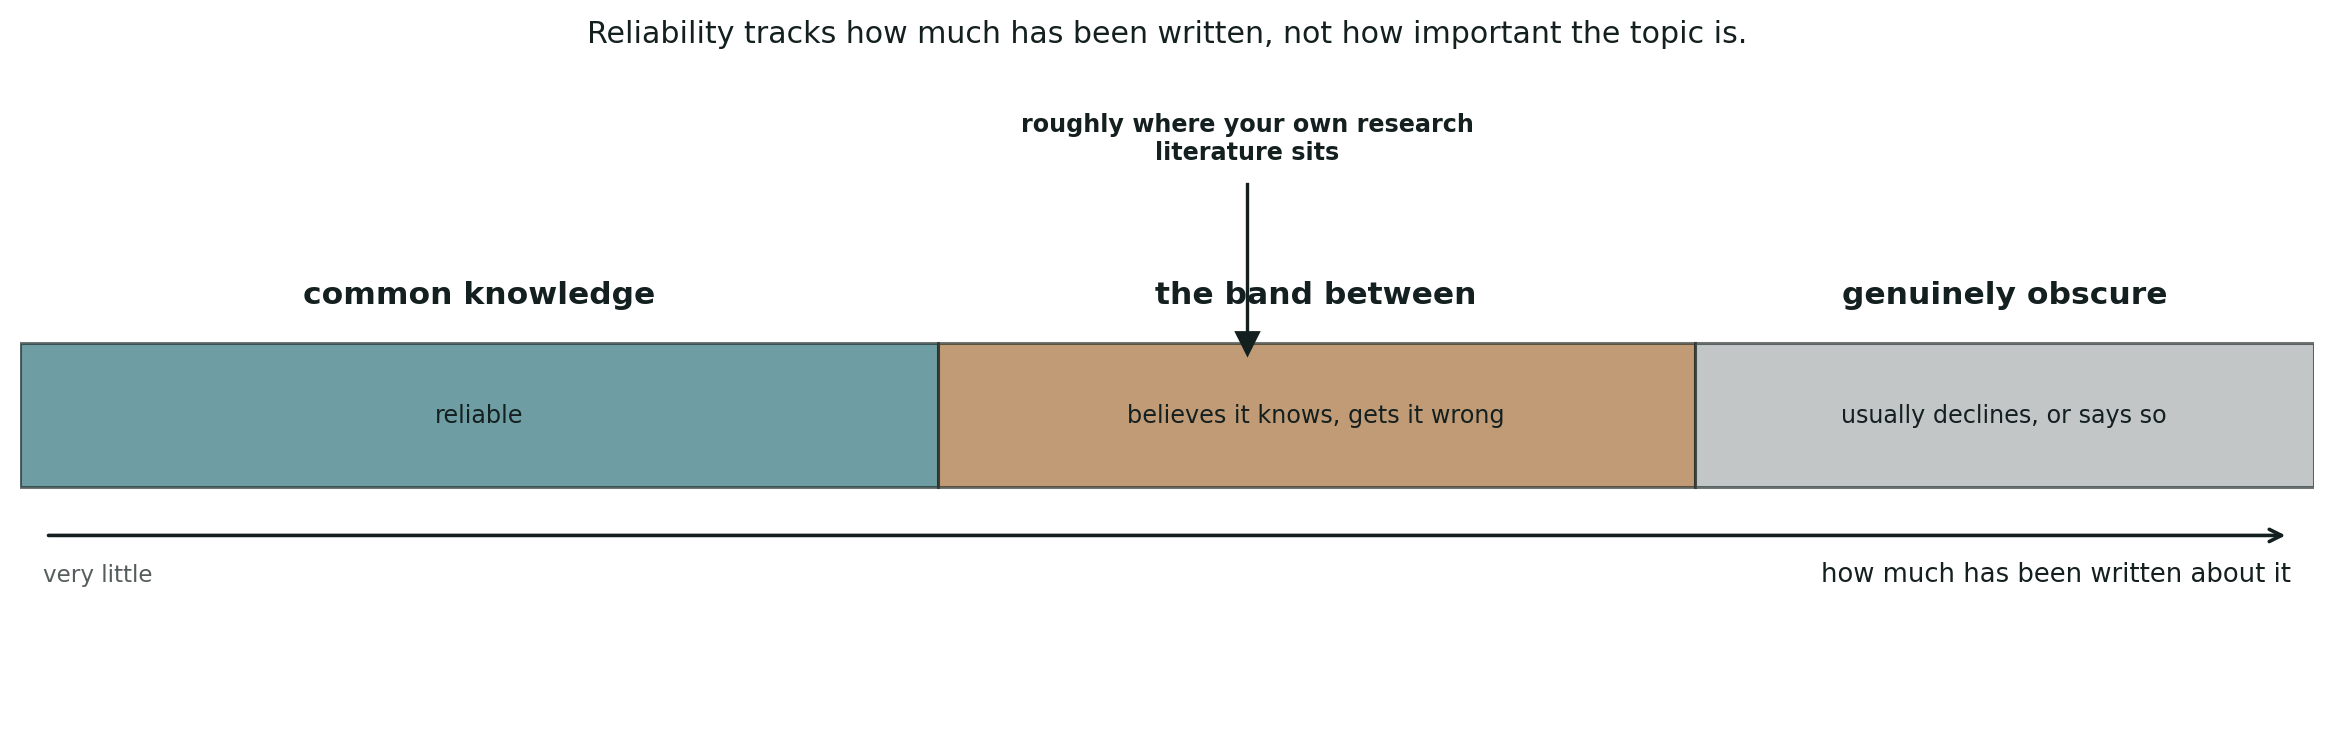
\includegraphics[height=38mm,width=\linewidth,keepaspectratio]{01-corpus-density}\end{center}
  \vspace{-0.6em}
  {\small The \kw{corpus} is the text training ran over. A prediction can be fluent and still
   wrong; what governs which is how much was written. \textcolor{uhocher}{TODO(verify)}}
  \provenance{definition}
\end{frame}
\note{%
This is the slide that makes the room care about tokens, and it is the hook for Chapter 5.\\[0.3em]
It behaves as though it had counted how often words appear together --- but it kept no counts. It
kept a fitted function. That distinction is why it can be fluent and wrong: a lookup table cannot
invent a plausible citation, and a fitted function can.\\[0.3em]
The practical version: you could not train a useful model for fluid-structure interaction on chat
transcripts. Do NOT suggest they shop for a domain-specific model instead --- someone will ask
which one, and there is no usable answer. The point is the corpus, and that their own field sits
in the middle band where the tool feels confident and is not.\\[0.3em]
This figure is reused by Chapter 5. Do not add Chapter 1 wording to it.}

% ---------------------------------------------------------------- 5
\begin{frame}{A model is numbers plus a program}
  \begin{center}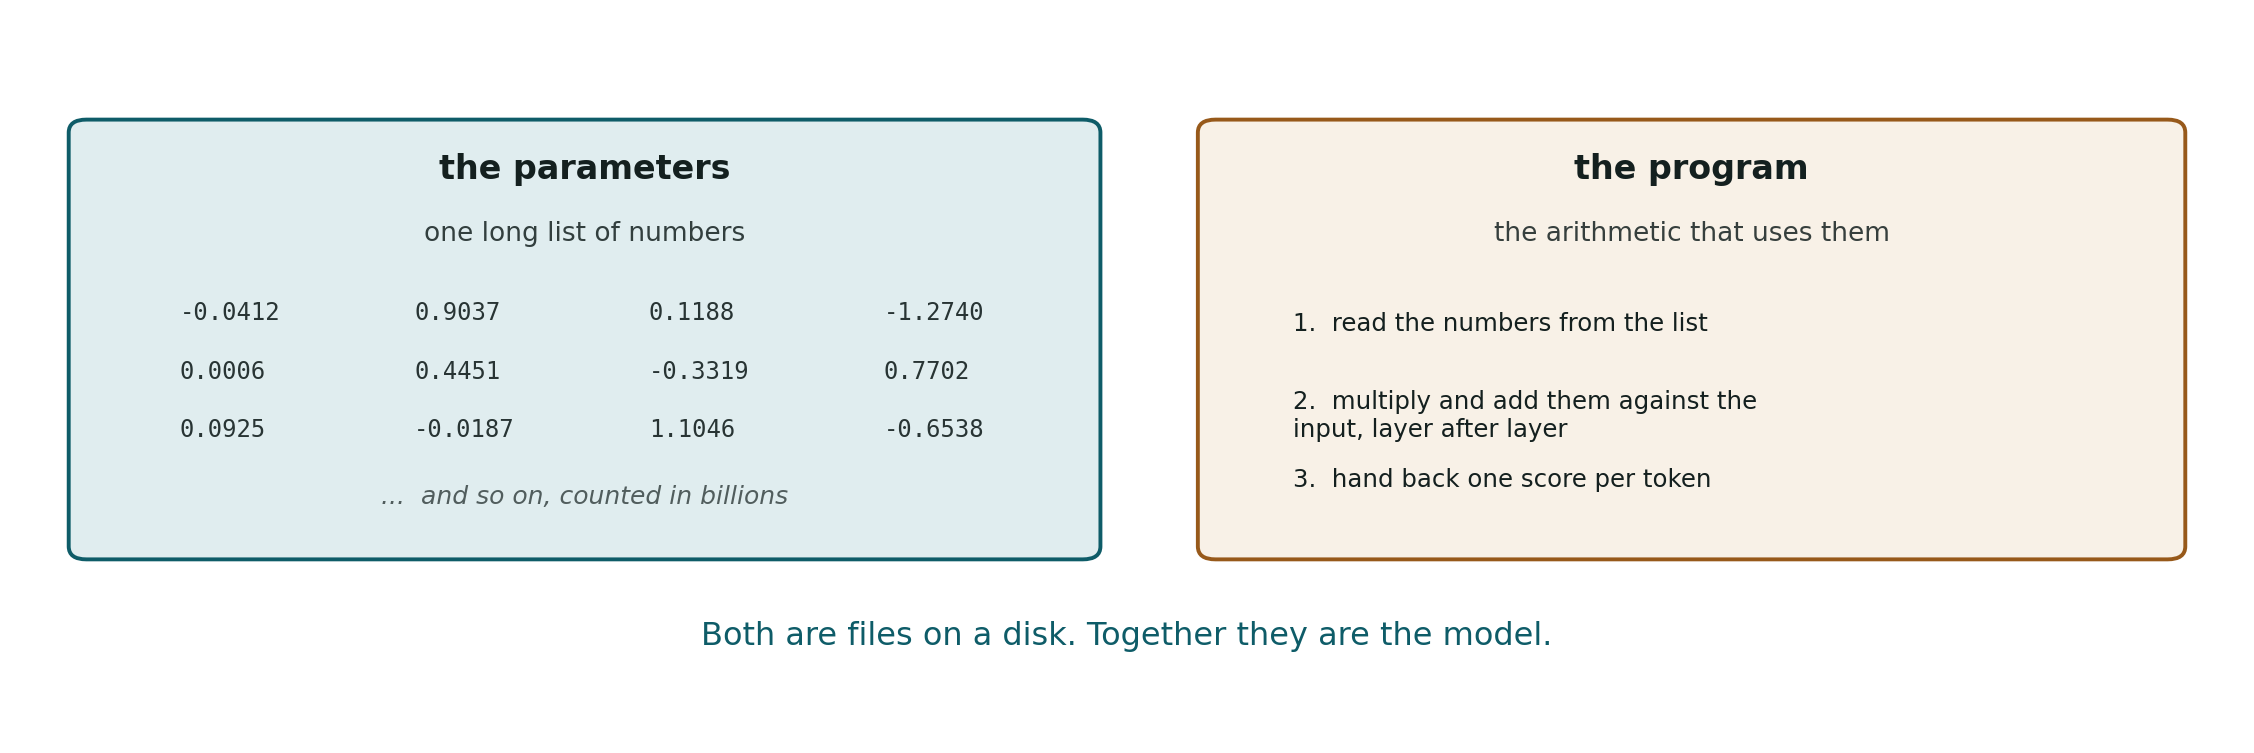
\includegraphics[height=34mm,width=\linewidth,keepaspectratio]{01-model-artefact}\end{center}
  \begin{columns}[t]
    \begin{column}{0.31\linewidth}\centering
      \kw{Parameters}\\[0.2em]{\small also \kw{weights}; \emph{fitted}, not designed}
    \end{column}
    \begin{column}{0.31\linewidth}\centering
      \kw{Network}\\[0.2em]{\small layered weighted sums}
    \end{column}
    \begin{column}{0.31\linewidth}\centering
      \kw{Size}\\[0.2em]{\small how many were fitted}
    \end{column}
  \end{columns}
  \provenance{definition}
\end{frame}
\note{%
This is what "I use Sonnet 5" actually names: one particular list of numbers, on a disk
somewhere, plus the program that evaluates it. Different name, different list.\\[0.3em]
The framing of a model as two files is Karpathy's. It costs one slide and it fixes the thing the
course was faulted for skipping.\\[0.3em]
Do not state a file size or a parameter count. Those are per-model claims and none is cited here.}

% ---------------------------------------------------------------- 6
\begin{frame}{Training set those numbers and then stopped}
  \begin{center}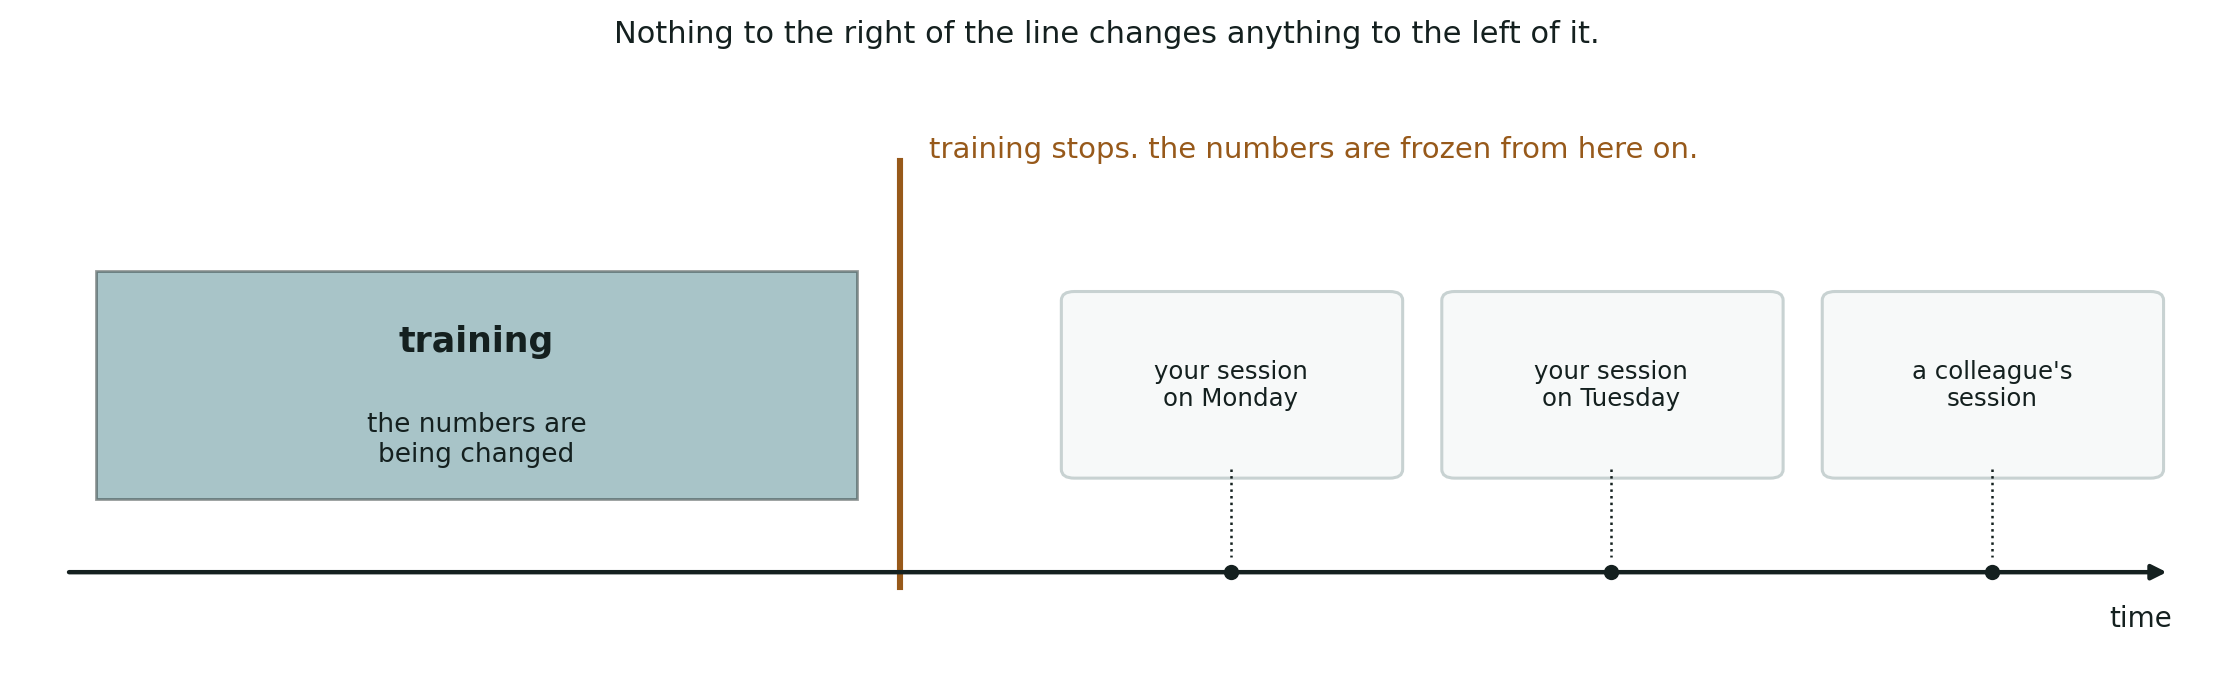
\includegraphics[height=27mm,width=\linewidth,keepaspectratio]{01-train-vs-run}\end{center}
  \begin{columns}[t]
    \begin{column}{0.31\linewidth}\centering
      \kw{Training}\\[0.2em]{\small the phase in which the numbers were changed}
    \end{column}
    \begin{column}{0.31\linewidth}\centering
      \kw{Inference}\\[0.2em]{\small running the finished numbers on your text}
    \end{column}
    \begin{column}{0.31\linewidth}\centering
      \kw{Knowledge cutoff}\\[0.2em]{\small the date training stopped}\\[0.5em]
      \kw{Session}\\[0.2em]{\small one continuous conversation}
    \end{column}
  \end{columns}
  \provenance{definition}
\end{frame}
\note{%
Everything the room will ever do happens to the right of the line. One \kw{session} is one
continuous conversation, from opening it to closing it.\\[0.3em]
The cutoff is a consequence of the process, not a policy about what to withhold.\\[0.3em]
Caveat: models are retrained and replaced. A given model's numbers never change; the model you
are pointed at can.}

% ---------------------------------------------------------------- 7
\begin{frame}{Training searches for the smallest total error}
  \begin{center}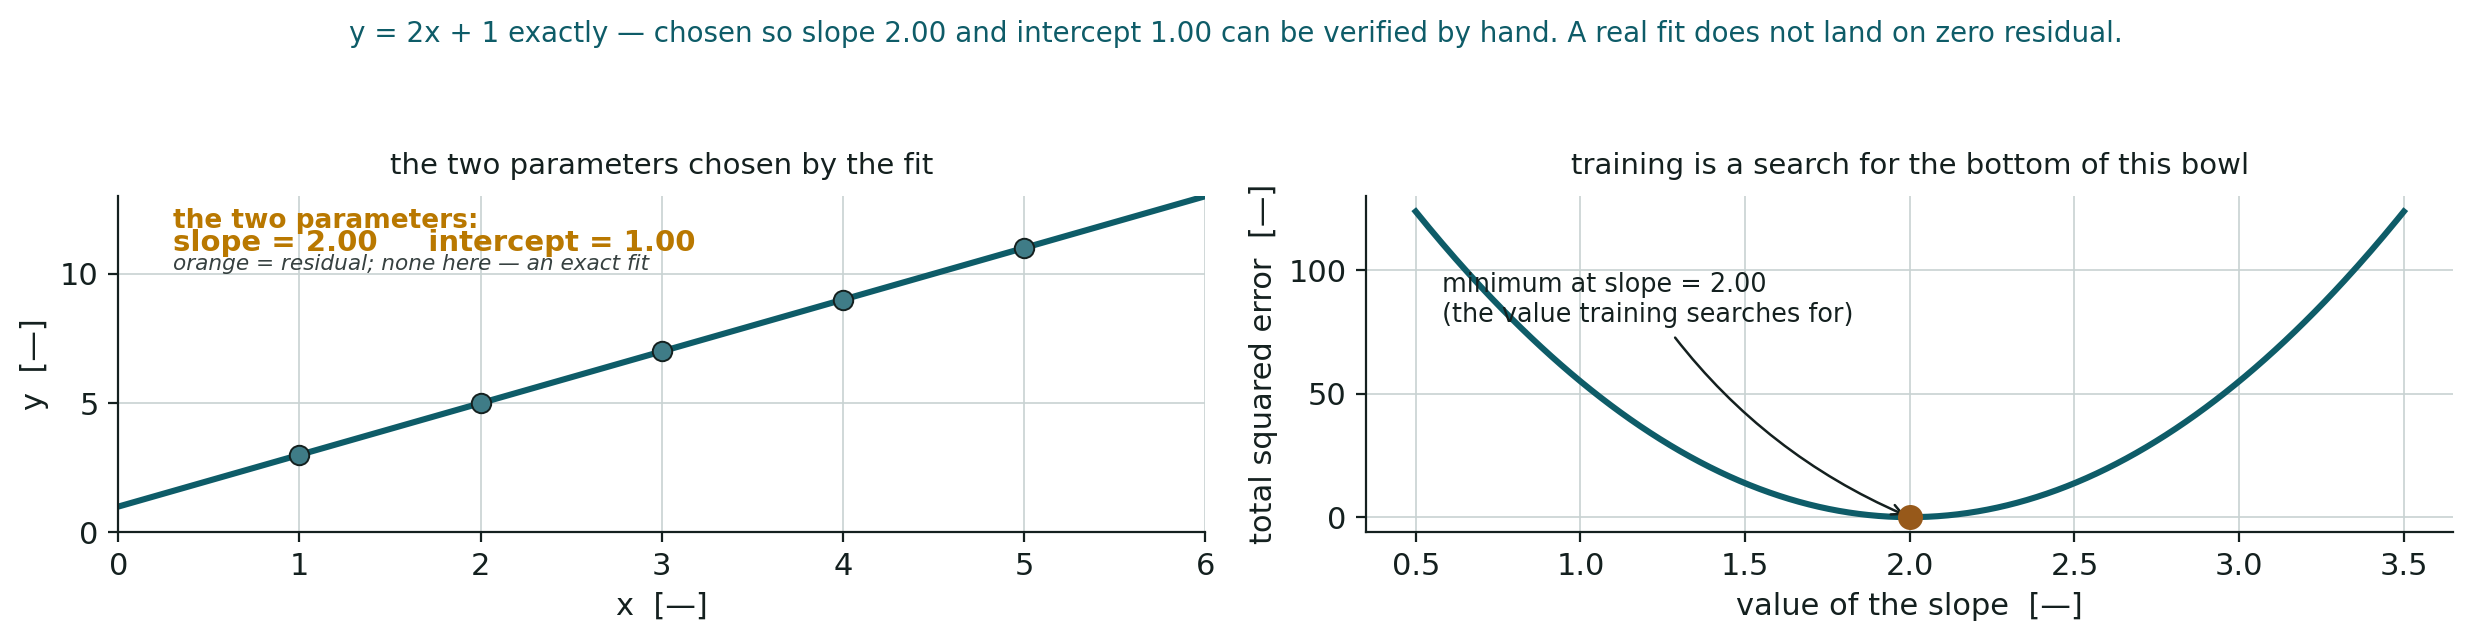
\includegraphics[height=33mm,width=\linewidth,keepaspectratio]{01-fitting}\end{center}
  {\small Two parameters here: \param{slope 2.00} and \param{intercept 1.00}. A language model
   runs the same kind of search over billions of them, with text as the data. There is no closed
   form, and it stops at a good enough set rather than the best possible.}
  \provenance{computed}
\end{frame}
\note{%
The discipline bridge. Everyone in the room has fitted a line. A model is a parameterised function
fitted to data by minimising an error, which is a sentence they can already check.\\[0.3em]
The numbers are deliberately round so the arithmetic can be followed live: y = 2x + 1 exactly, so
the residuals are zero and the fit is checkable by eye. Say that a real fit has residuals and this
one is clean on purpose.\\[0.3em]
A concrete-mix analogy works well for what a weight IS --- 0.2 water, 0.5 cement, 0.3 aggregate,
proportions that combine inputs into an output. State its limit in the same breath: you choose a
mix and it sums to one; a model's weights are fitted, can be negative, and there are billions.
Naming the limit of an analogy is the discipline this course teaches.\\[0.3em]
Caveat: the right-hand panel varies one parameter. A real run searches a space with billions of
dimensions, and the bowl is a one-dimensional slice of it.}

% ---------------------------------------------------------------- 8   (was 9)
\begin{frame}{Training changed the numbers, nothing else}
  \begin{center}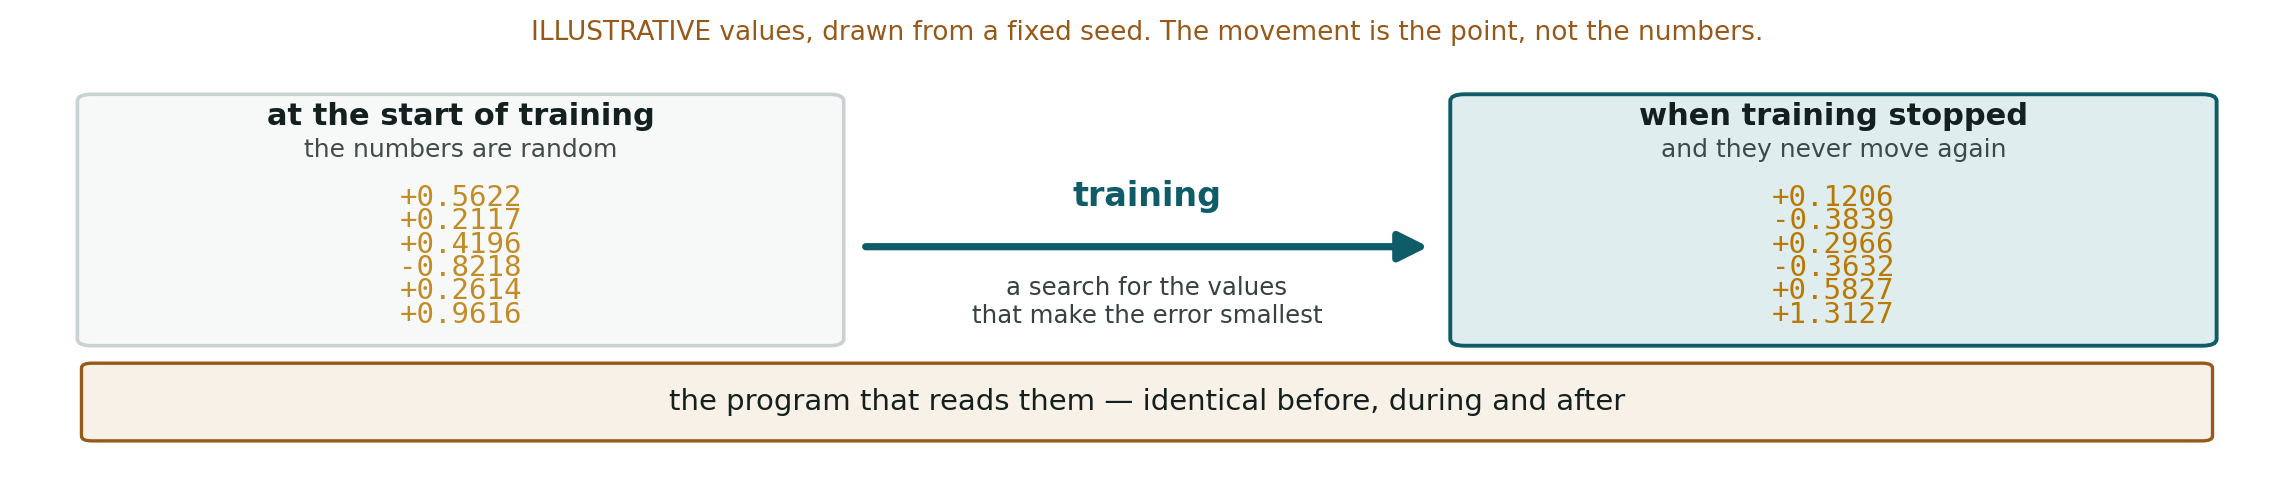
\includegraphics[height=31mm,width=\linewidth,keepaspectratio]{01-what-training-changed}\end{center}
  \begin{columns}[t]
    \begin{column}{0.31\linewidth}\centering
      \kw{Neural network}\\[0.2em]{\small layers of multiply-and-add, named after a biological analogy}
    \end{column}
    \begin{column}{0.31\linewidth}\centering
      \kw{Learning}\\[0.2em]{\small the search you just watched}
    \end{column}
    \begin{column}{0.31\linewidth}\centering
      \kw{The brain comparison}\\[0.2em]{\small correlational; the appendix carries what it establishes}
    \end{column}
  \end{columns}
  \citesource{schrimpf2021,hadidi2026}
\end{frame}
\note{%
Answers "is it like a brain?" once, at the point the room reaches for it --- they have just been
told the thing is a neural network that learns --- and closes it. No later chapter has to unteach
an analogy this course taught.\\[0.3em]
The numbers started as noise. Whatever the system does, it acquired by a search over those numbers
against a measure of error, and that is the whole of what training is.\\[0.3em]
The three facts behind the citation, if pressed: the encoding-model work reports predictivity
normalised by noise ceilings of 0.32, 0.17 and 0.20 across its three datasets; the
predictive-processing conclusion is a between-model correlation rather than something measured
inside a brain; and Idan Blank co-authored both the original paper and the later re-analysis.\\[0.3em]
Do not say the comparison has been refuted. It has been qualified by its own authors, which is a
different and more useful thing.\\[0.3em]
Chapter 8 is now the appendix deck --- distributed, not presented.}

% ---------------------------------------------------------------- 9   (was 10)
\begin{frame}{Text becomes numbers, then scores, then text}
  \begin{center}
\fitwidth{%
    \begin{tikzpicture}[node distance=5mm]
    \node[uhbox]                        (a) {your text};
    \node[uhwide, right=of a]           (b) {cut into tokens,\\each one an integer};
    \node[uhhi,   right=of b]           (c) {the network};
    \node[uhwide, right=of c]           (d) {one score for\\every token};
    \node[uhamber,right=of d]           (e) {choose one};
    \node[uhbox,  right=of e]           (f) {the text\\you see};
    \draw[uhar] (a)--(b); \draw[uhar] (b)--(c); \draw[uhar] (c)--(d);
    \draw[uhar] (d)--(e); \draw[uhar] (e)--(f);
    \draw[uhar] (e.south) -- ++(0,-5mm) -| node[pos=0.25,below,font=\scriptsize\itshape]
      {append it and run again} (b.south);
  \end{tikzpicture}}
  \end{center}
  {\small We walk this left to right. Some boxes take more than one slide. \kw{Token} is a chunk of characters from a
   fixed list, defined next.}
  \provenance{definition}
\end{frame}
\note{%
The map. Preview the whole data path before explaining any stage, so every later detail has
somewhere to attach. The structure is 3Blue1Brown's and it is the best answer to a room holding
both beginners and people who already know some of this.\\[0.3em]
Say explicitly: we walk this left to right and we do not jump about. The previous version of this
chapter did, and it was the loudest complaint in review.\\[0.3em]
The arrow labelled "append it and run again" is the whole reason the answer arrives a piece at a
time.}

% ---------------------------------------------------------------- 10   (was 12)
\begin{frame}{Tokens come from a fixed list}
  \begin{center}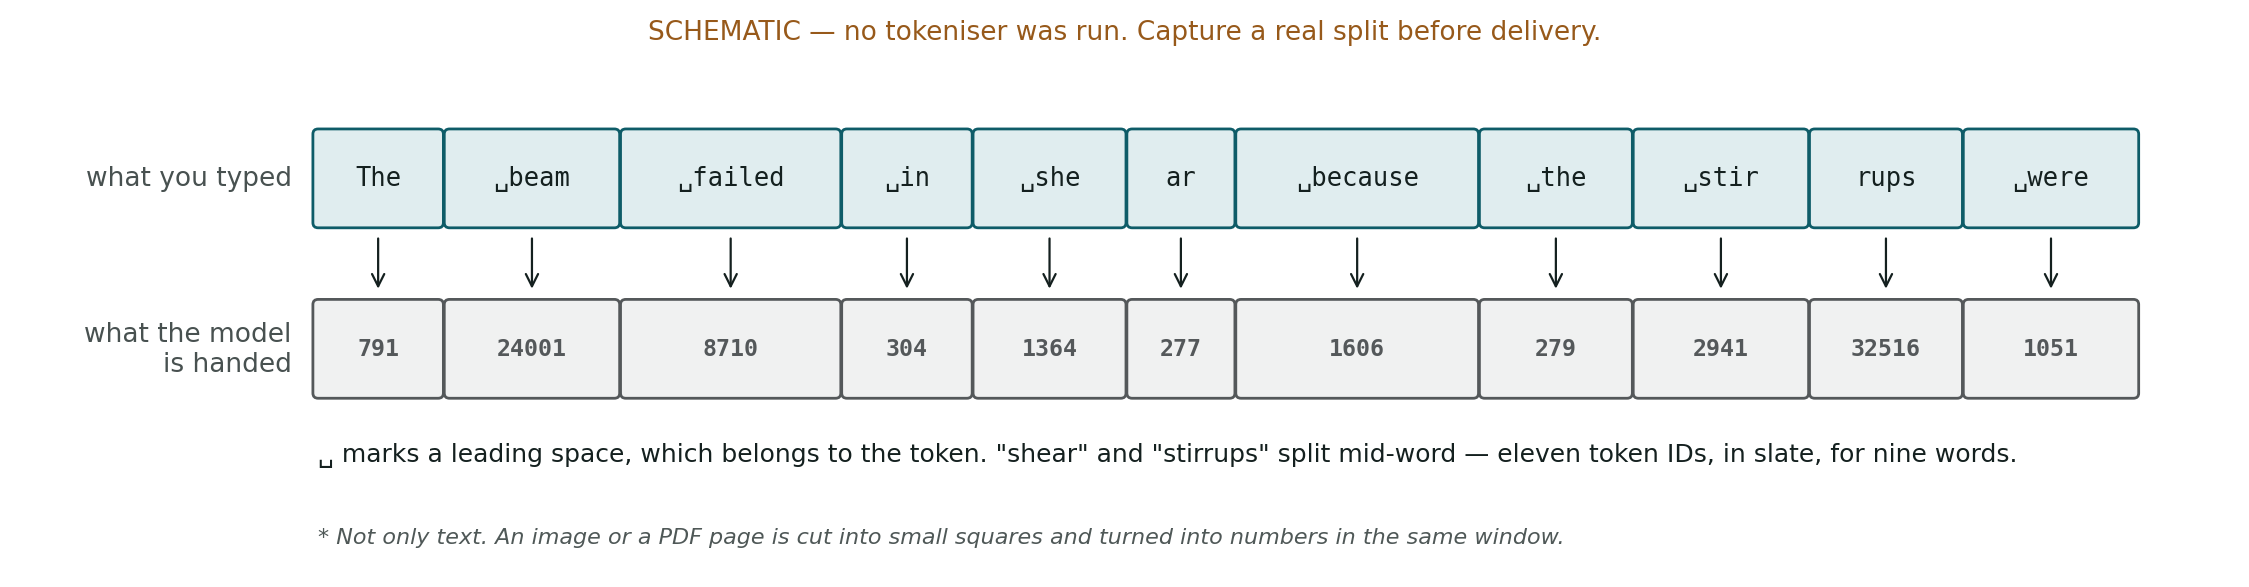
\includegraphics[height=29mm,width=\linewidth,keepaspectratio]{01-tokens}\end{center}
  \begin{columns}[t]
    \begin{column}{0.31\linewidth}\centering
      \kw{The vocabulary}\\[0.2em]{\small the model's list, not English}
    \end{column}
    \begin{column}{0.31\linewidth}\centering
      \kw{Token IDs}\\[0.2em]{\small \tokid{labels}, not quantities}\\[0.4em]
      {\footnotesize \emph{shear} may split as \emph{she}+\emph{ar}: common letter runs, not words}
    \end{column}
    \begin{column}{0.31\linewidth}\centering
      \kw{No letters}\\[0.2em]{\small the network is handed integers}
    \end{column}
  \end{columns}
  \provenance{schematic}
\end{frame}
\note{%
The distinction that stops the room conflating four kinds of number: adding two \tokid{token IDs}
is meaningless, adding two \param{parameters} is not. A token ID is a label with no magnitude. Say
it here and the colour code carries it for the rest of the chapter.\\[0.3em]
The list is built before training and never changes afterwards. A word not in it is split into
pieces that are, which is why a model can produce words nobody ever wrote down.\\[0.3em]
The asterisk on the figure: not only text. An image or a PDF page is cut into small squares and
turned into numbers in the same window. They will paste a photograph of a cracked specimen in week
one, and this is the line that stops the next slide looking false when they do.\\[0.3em]
TODO(capture): run a real tokeniser on this sentence and on a MATLAB snippet. The figure says
SCHEMATIC until that is done.}

% ---------------------------------------------------------------- 11   (was 13)
\begin{frame}{Token count follows frequency, not length}
  \begin{center}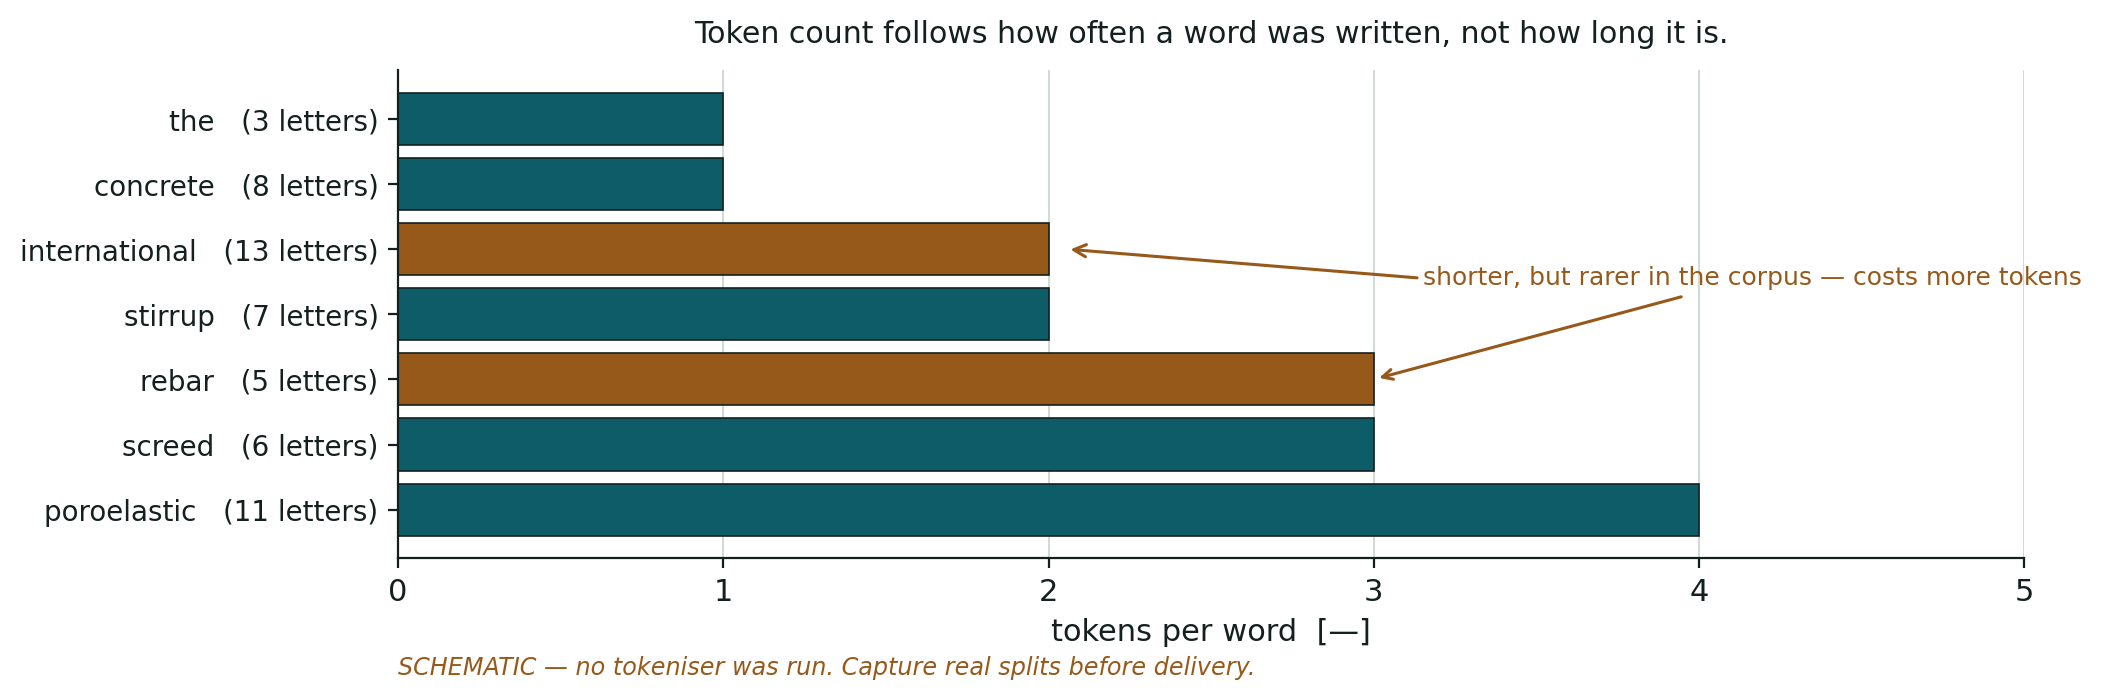
\includegraphics[height=38mm,width=\linewidth,keepaspectratio]{01-token-cost}\end{center}
  \begin{columns}[t]
    \begin{column}{0.31\linewidth}\centering\kw{Billed}\\[0.2em]{\small per token}\end{column}
    \begin{column}{0.31\linewidth}\centering\kw{Context limit}\\[0.2em]{\small counted in tokens}\end{column}
    \begin{column}{0.31\linewidth}\centering\kw{Speed}\\[0.2em]{\small quoted per token}\end{column}
  \end{columns}
  \provenance{schematic}
\end{frame}
\note{%
A short rare word can cost more tokens than a long common one. Point at that row --- it is the
whole slide. The rule is frequency in the training corpus, not length, and the previous version of
this figure taught the wrong one.\\[0.3em]
Practical effect: a page of your writing costs more tokens than a page of a newspaper. Nothing is
wrong when that happens.\\[0.3em]
This is the cost thread's first appearance. Chapter 7 prices it and Chapter 13 bills it.}

% ---------------------------------------------------------------- 12   (was 8)
\begin{frame}{Training minimises surprise at the next token}
  \begin{center}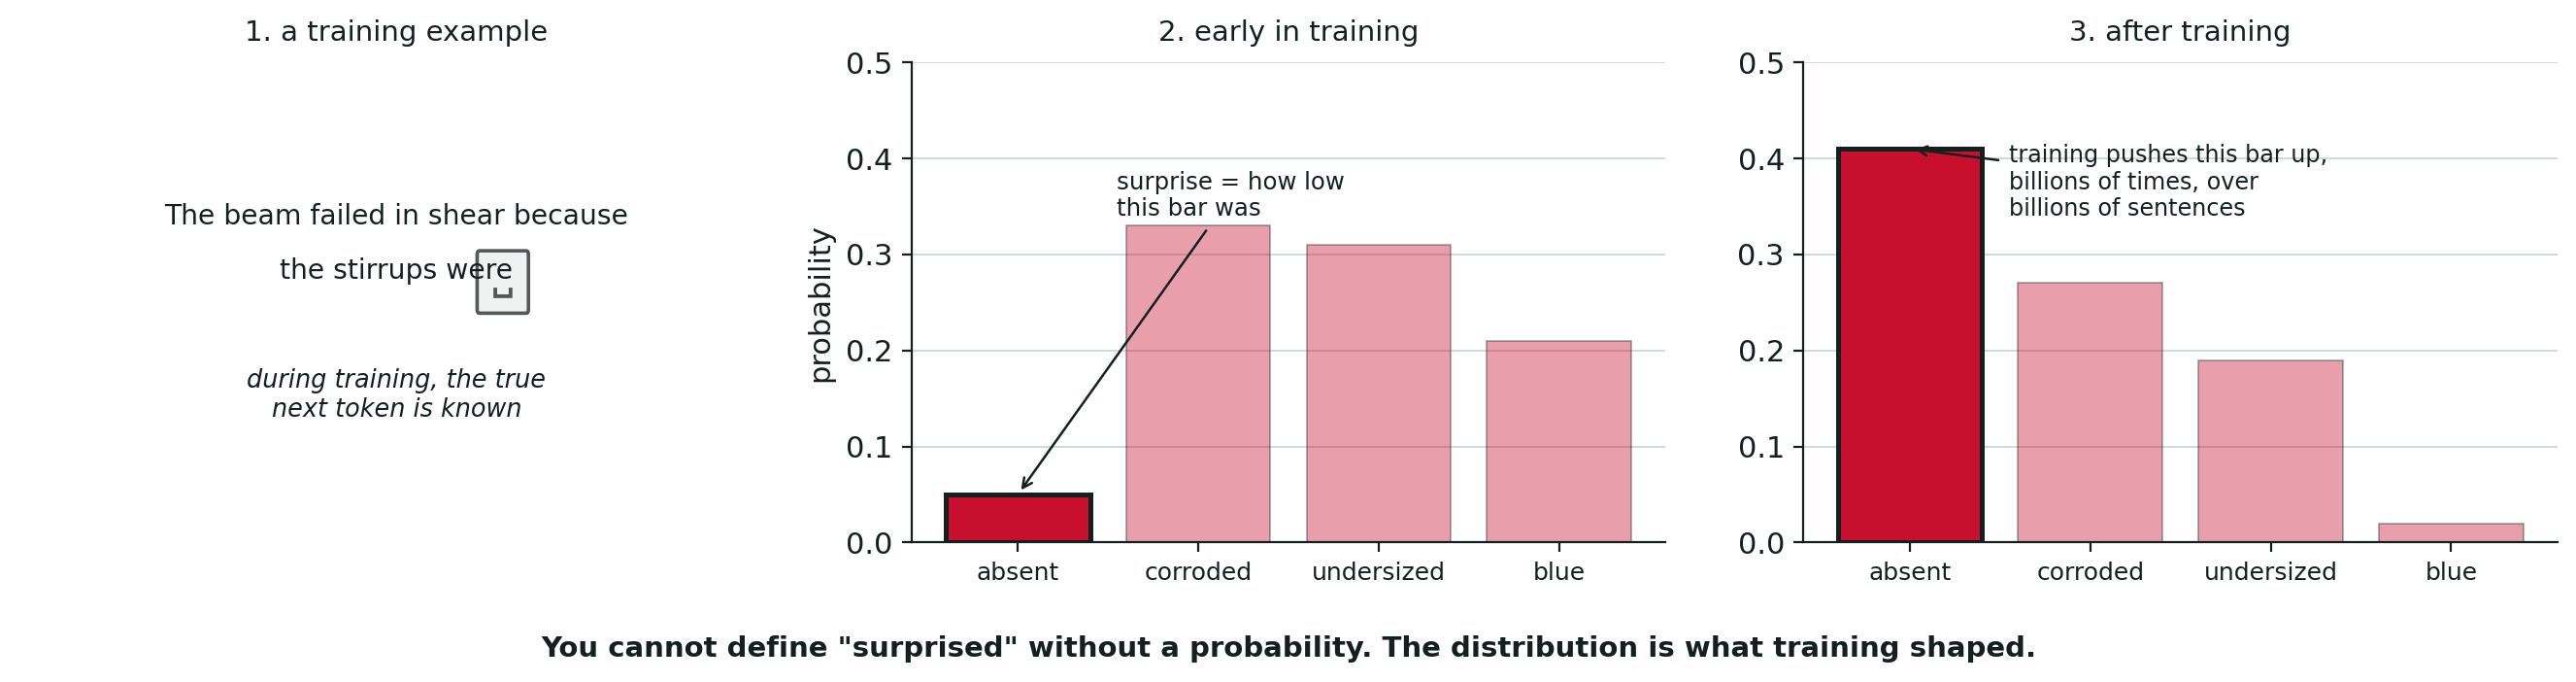
\includegraphics[height=38mm,width=\linewidth,keepaspectratio]{01-surprise}\end{center}
  {\small \kw{Surprise} is $-\log \mprob{p}$ for the token that actually came next, so the thing training
   shaped is a distribution over every \kw{token} that could come next.}
  \provenance{derived}
\end{frame}
\note{%
THIS IS THE SLIDE THE CHAPTER WAS MISSING, and it is the bridge from deterministic to
probabilistic. Deliver it slowly.\\[0.3em]
The chain, said out loud: training minimises surprise at the true next token, so the output has to
be a distribution --- there would be nothing to minimise otherwise. For a fixed input that
distribution is computed deterministically, the same every time. Take its maximum every time and
the text loops. So a token is drawn from it instead. Therefore two runs of the same prompt differ.
Every step has a reason; nothing is asserted.\\[0.3em]
An engineering analogy that works: cast fifty specimens from one mix and you get fifty compressive
strengths, and you infer a distribution from them. Name the joint where it fails, because it is
worth teaching --- with fifty cylinders you discover the distribution by testing fifty. The model
computes the distribution first, in one pass, and then throws almost all of it away by picking one
token. You never see it unless you look.\\[0.3em]
That is also why Chapter 4 makes you run the same prompt several times: you only ever observe the
picks, never the distribution.\\[0.3em]
Do NOT link this to temperature. Temperature is a sampler setting applied at inference, after the
numbers are frozen. It has nothing to do with the minimisation.\\[0.3em]
If asked about local minima and random starts: yes, training is genuinely stochastic, and two
training runs give different weights. That explains why one model differs from another, and it is
Chapter 4's reason for recording the model ID. It is NOT the reason the same prompt gives two
answers today --- those weights were frozen before anyone here touched the tool.}

% ---------------------------------------------------------------- 13   (was 14)
\begin{frame}{The network returns one score per token}
  \begin{center}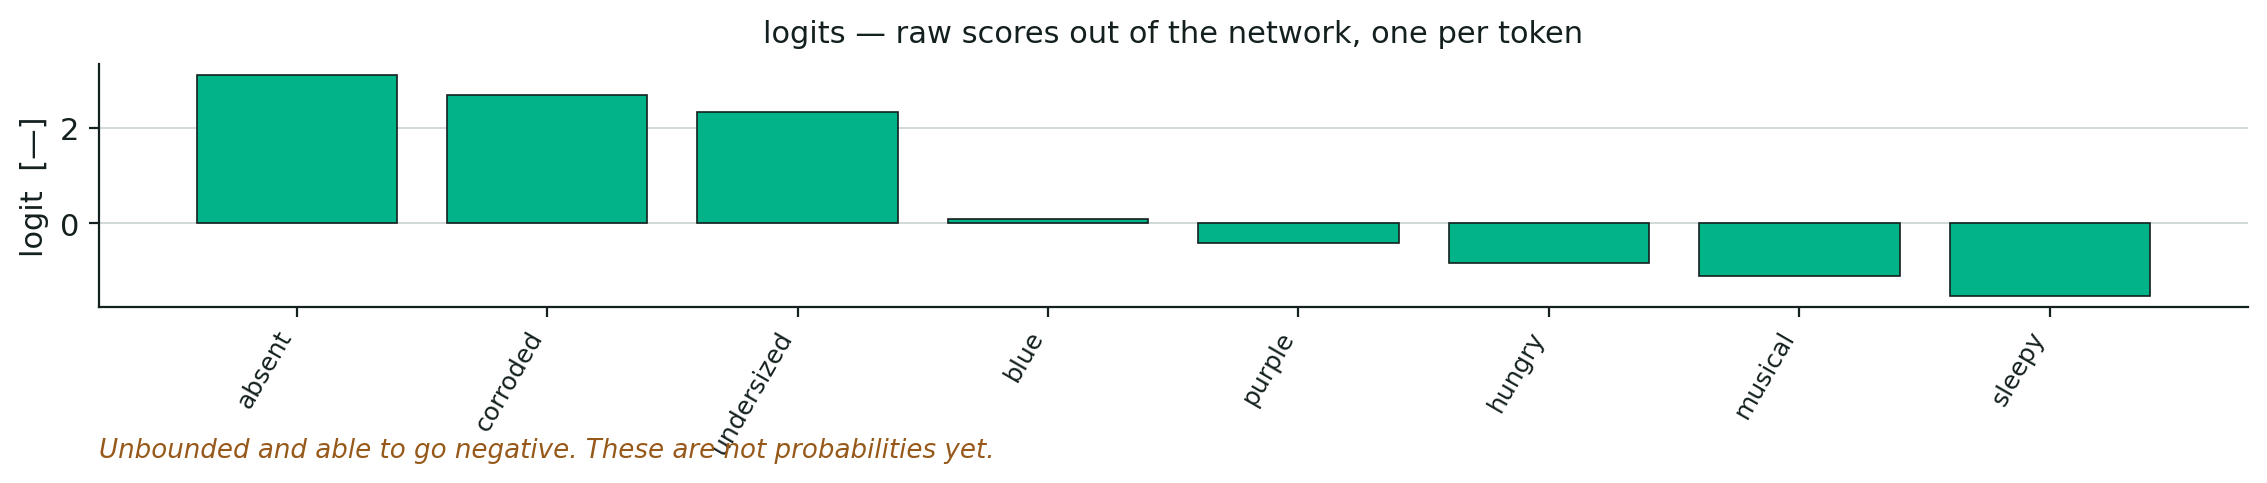
\includegraphics[height=33mm,width=\linewidth,keepaspectratio]{01-logits}\end{center}
  {\small A \logit{logit} is a raw score for one token, unbounded and able to go negative. One run
   of the network over the window is one \kw{pass}. These are not probabilities yet, and the
   remainder.}
  \provenance{definition}
\end{frame}
\note{%
The reason, and it is the point of the headline: the program is a fixed sequence of
multiplications and additions. It has no step that decides on an answer and writes it out. The only
thing it can produce is numbers, so an answer has to be assembled from what those numbers rank.\\[0.3em]
Note the colours doing work here: \logit{logits} in teal come out of the network,
\prob{probabilities} in red come out of the next slide. Different quantities, different colours,
every time they appear.\\[0.3em]
Values are illustrative and the figure says so.}

% ---------------------------------------------------------------- 14   (was 15)
\begin{frame}{Attention decides which earlier tokens matter}
  \begin{center}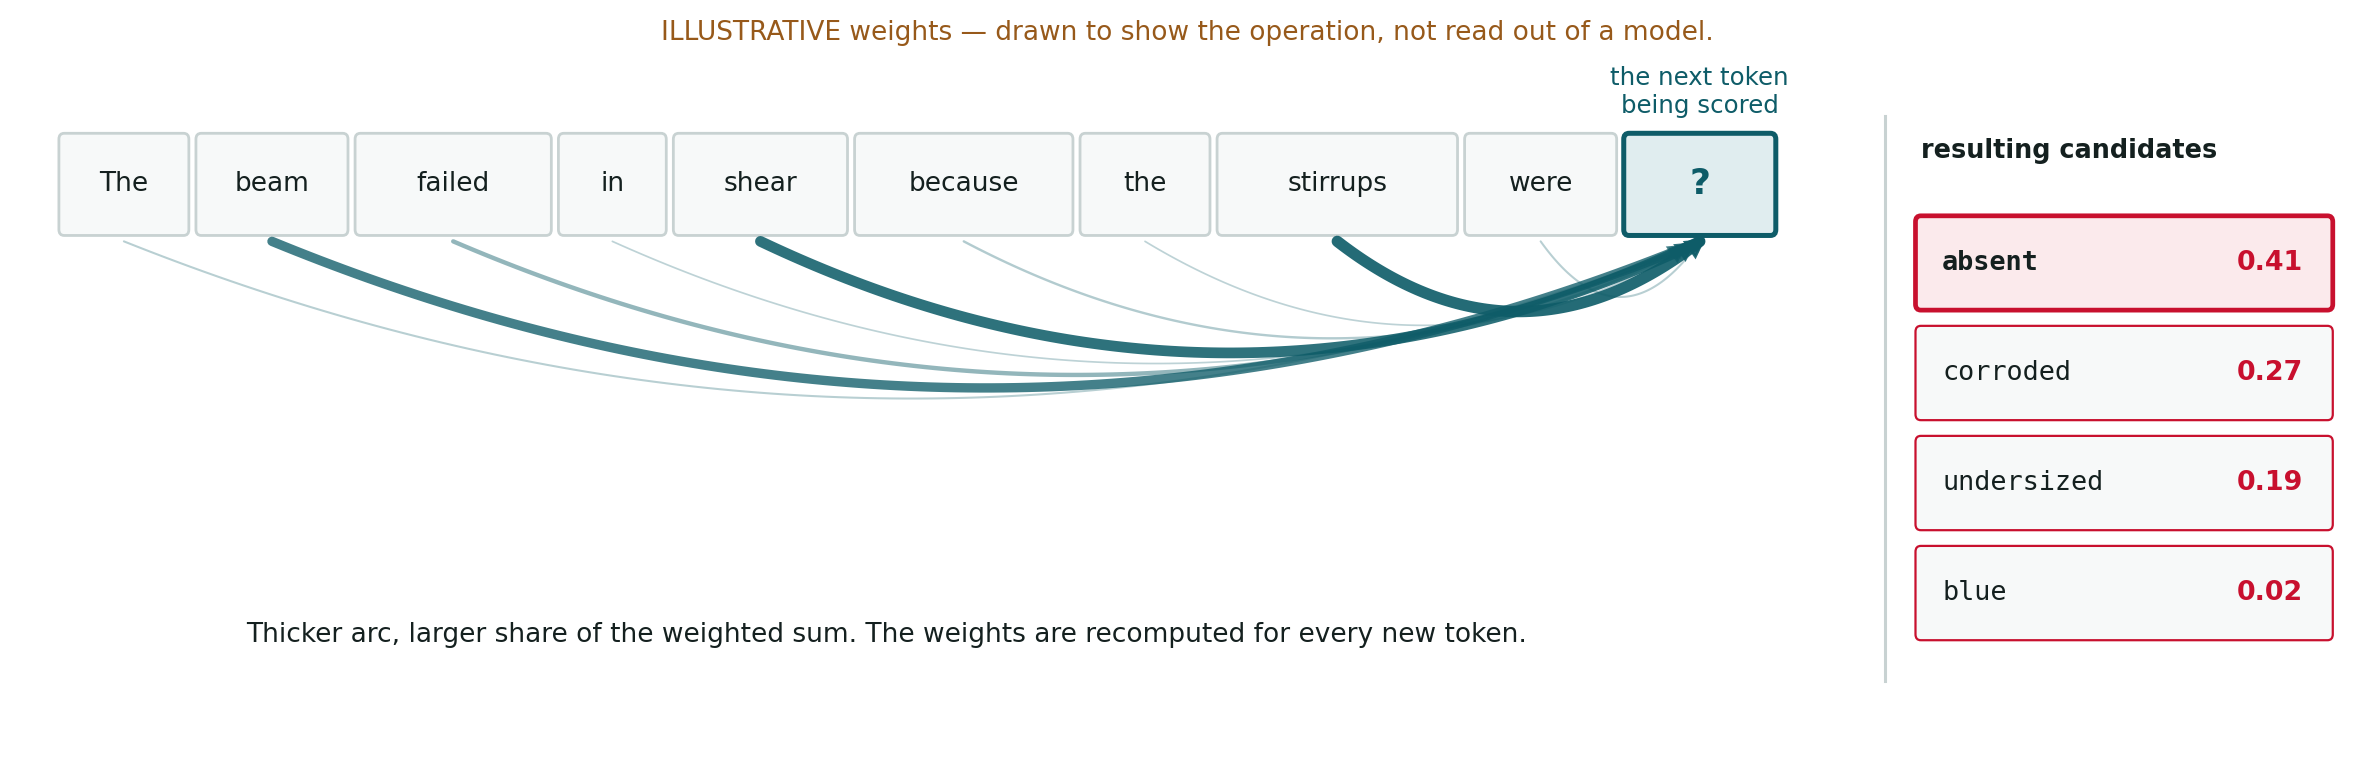
\includegraphics[height=35mm,width=\linewidth,keepaspectratio]{01-attention}\end{center}
  \animatable{A3}{1600 $\times$ 600 px}
  {\small A \kw{weighted sum}: the weight on each earlier position comes from comparing it against
   the position being scored. A \kw{transformer} is the arrangement of that arithmetic.}
  \citesource{vaswani2017}
\end{frame}
\note{%
Answers the question the previous slide raises: how can a score for the next token depend on a word
twenty tokens back.\\[0.3em]
Say plainly that it is not a chain. Every token in the window is used to score the next one, all of
them, together, every pass. If the room holds a chain model --- each word influencing the one after
it --- then this slide, the position effects in Chapter 5, and the whole point of a context window
all stop making sense.\\[0.3em]
The paper's exact wording if anyone asks: attention maps "a query and a set of key-value pairs to
an output", computed as "a weighted sum of the values, where the weight assigned to each value is
computed by a compatibility function of the query with the corresponding key". Those three role
names are kept off the slide on purpose --- the course never uses them again, and naming them would
leave three terms undefined to save nothing.\\[0.3em]
Scope: one sentence and one diagram. How the weights are computed, multi-head attention and
positional encoding are all excluded, because none of them changes a decision anyone here makes.\\[0.3em]
The arc thicknesses are drawn to show the operation. They were not extracted from a model.}

% ---------------------------------------------------------------- 15   (was 16)
\begin{frame}{Softmax turns scores into probabilities}
  \vspace{1em}
  \begin{columns}[c]
    \begin{column}{0.52\linewidth}
      \[ \mprob{p_i} \;=\; \frac{\exp\!\big(\overbrace{\mlogit{z_i}}^{\text{score for token } i}\big/\underbrace{T}_{\text{temperature}}\big)}
         {\underbrace{\sum_j \exp(\mlogit{z_j}/T)}_{\substack{\text{sum over every token,}\\ \text{so the result adds to } 1}}} \]
      \vspace{0.3em}
      {\footnotesize As $T \to 0$ the top score wins outright. \kw{$T=0$ means take the
       maximum}, not divide by zero.}
    \end{column}
    \begin{column}{0.44\linewidth}
      {\small \kw{Worked case}, two candidates only, so the sum checks by hand.}
      \[ \mlogit{z_{\text{absent}}} = \ln 0.41 \qquad \mlogit{z_{\text{corroded}}} = \ln 0.27 \]
      \[ \mprob{p} = \frac{0.41}{0.41+0.27} = \mprob{0.603} \]
      {\small Two in the denominator gives \mprob{0.603}. Over the whole vocabulary it is
       \mprob{0.41}, which is the number the figures carry. All quantities dimensionless.}
    \end{column}
  \end{columns}
  \provenance{computed}
\end{frame}
\note{%
The only equation in the chapter, and the one the room can check by hand in ten seconds.
Because the scores are written as $\ln p$, the exponentials are the probabilities themselves:
$0.41$ and $0.27$, sum $0.68$, ratio $0.603$.\\[0.3em]
Say why it is restricted to two candidates: the real denominator runs over the whole vocabulary and
cannot be shown. Two is enough to check the arithmetic.\\[0.3em]
State the two denominators out loud. Restricted to two candidates the answer is 0.603; over the
whole vocabulary it is 0.41. Both are correct and they are answers to different questions. The
temperature sweep is shown as a curve on the temperature frame, not here.\\[0.3em]
Worth naming: the form is the Boltzmann distribution with the score standing in for negative energy
over kT. Several people in the room will recognise it.}

% ---------------------------------------------------------------- 16   (was 17)
\begin{frame}{Always taking the top token repeats}
  \slotF{temperature zero, run long enough that the output falls into a loop}

  {\small Taking the top token every time is \kw{greedy decoding}. It is observed to fall into
   loops: once a phrase appears, it raises the probability of its own continuation.
   \textcolor{uhocher}{TODO(cite)}}
  \provenance{observation}
\end{frame}
\note{%
The objective shown breaking. Stating what a system optimises and then showing it fail is the move
every reviewed explainer uses, and it is what stops next-token prediction sounding either trivial or
magical.\\[0.3em]
This slide comes BEFORE sampling on purpose. The previous version introduced the sampler first and
explained why it was needed two slides later, which is backwards.\\[0.3em]
TODO(capture): the recording is the evidence this slide is built on. Without it the slide argues a
mechanism it never demonstrates, and that is exactly what the review flagged.\\[0.3em]
If the recording does not loop --- some models resist repetition --- that is a result, not a failed
take. Show it and narrate the difference between "it was patched" and "it is fixed", which is the
policy Chapter 6 already uses for its demo.}

% ---------------------------------------------------------------- 17   (was 18)
\begin{frame}{The token is drawn, not taken}
  \begin{center}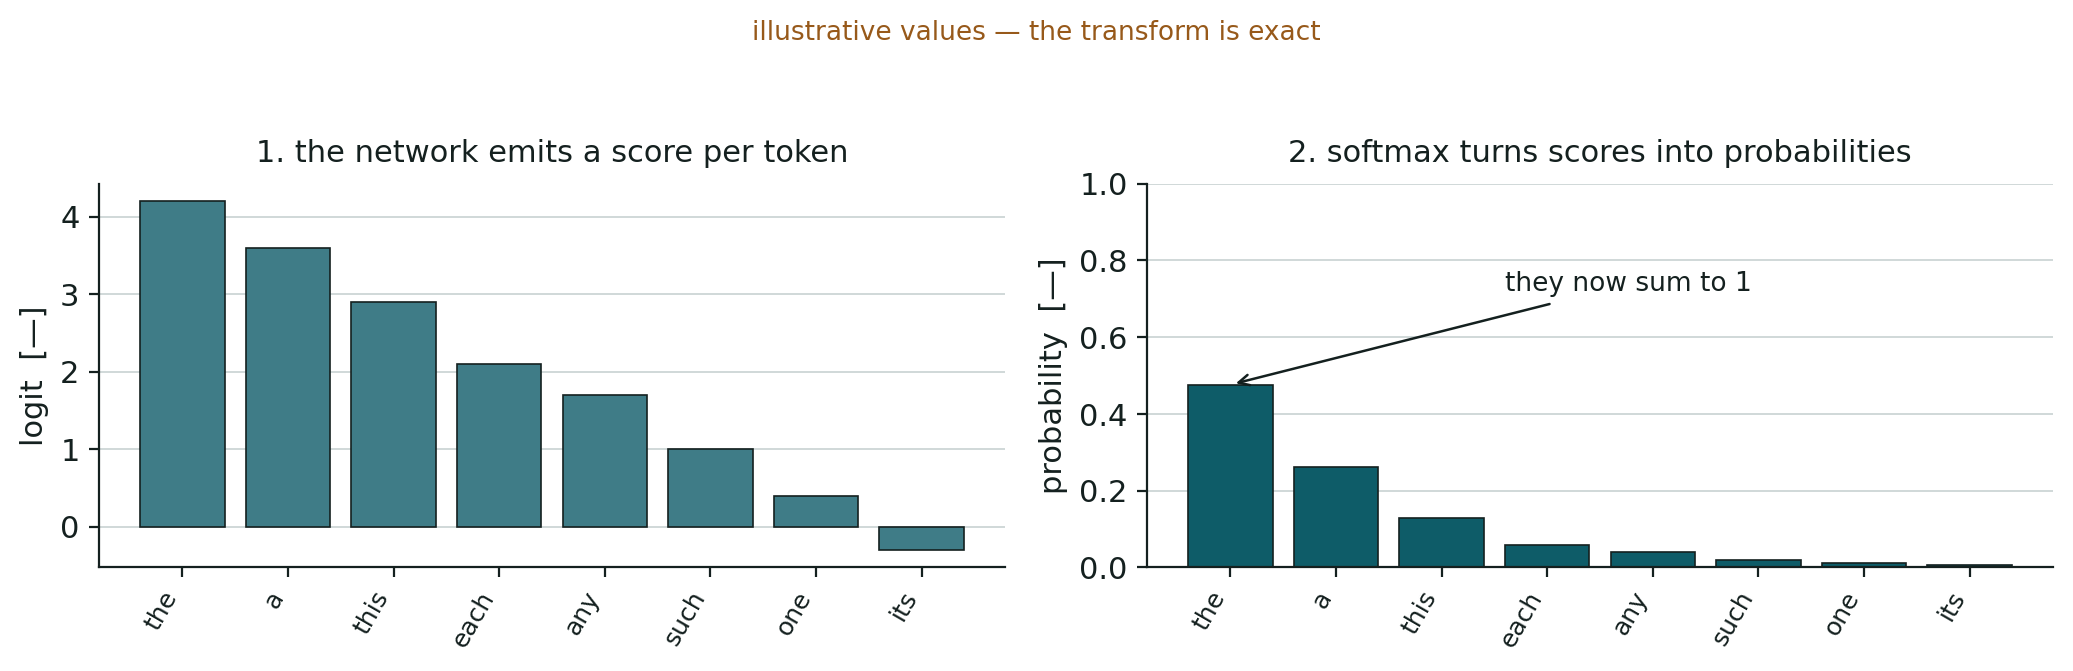
\includegraphics[height=38mm,width=\linewidth,keepaspectratio]{01-scores}\end{center}
  \animatable{A4}{1600 $\times$ 600 px --- the bars must be identical on every draw}
  {\small The bars are computed from the frozen numbers and never change. The \prob{draw} does.}
  \provenance{derived}
\end{frame}
\note{%
The resolution to the previous slide, and the single most important idea in the chapter.\\[0.3em]
The bars do not move. That is the whole point --- if the animation shows them shifting between
draws it teaches that the model is unstable, which is the reverse of the lesson.\\[0.3em]
Setting temperature to zero takes the top-scoring token every time and gives you back the previous
slide. Chapter 4 uses that.\\[0.3em]
Honest caveat: identical scores assume identical input and the same model version. On a hosted
service the hardware and the way requests are grouped on the server can perturb the arithmetic
slightly. What you actually see is dominated by the draw.}

% ---------------------------------------------------------------- 18   (was 19)
\begin{frame}{Temperature sets how sharply the top score wins}
  \begin{columns}[c]
    \begin{column}{0.53\linewidth}
      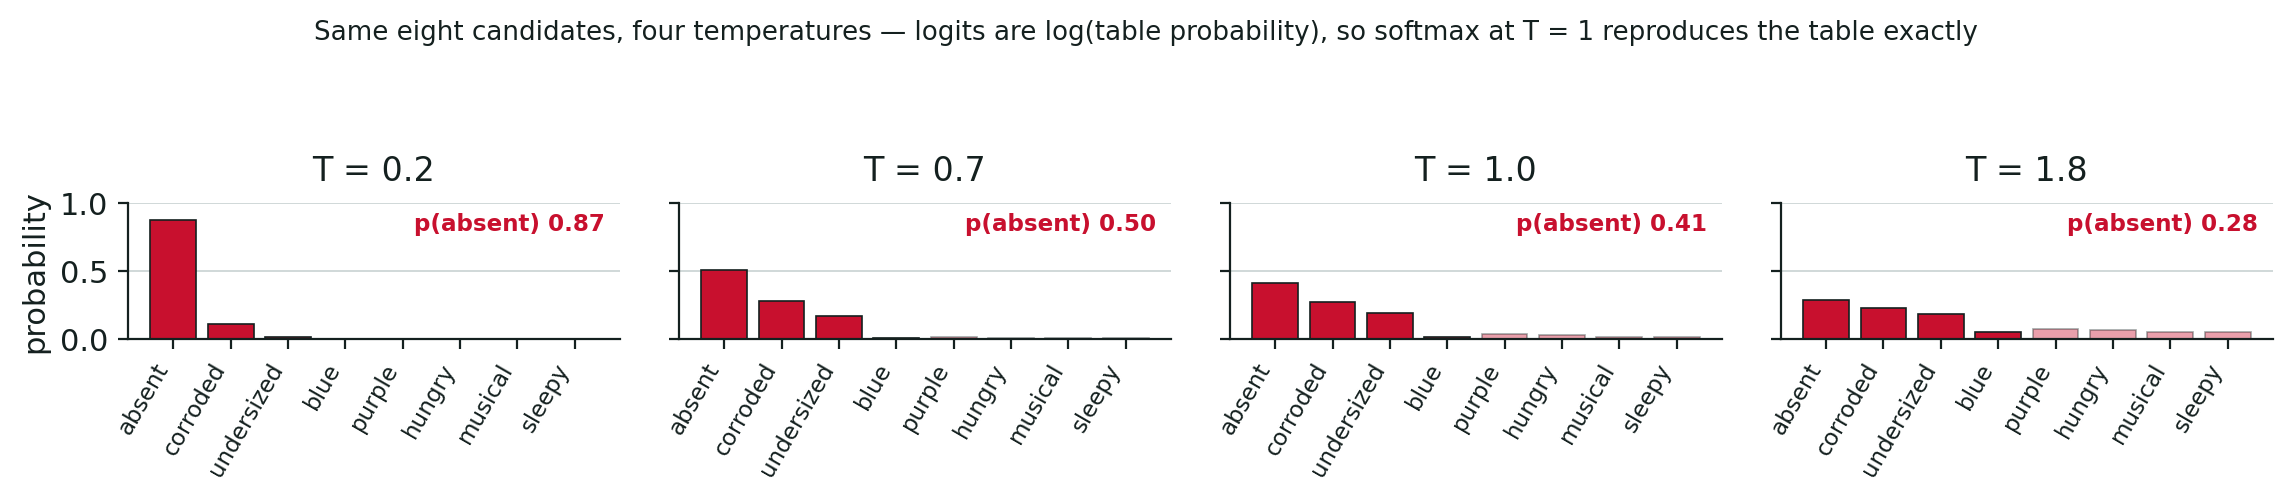
\includegraphics[height=30mm,width=\linewidth,keepaspectratio]{01-temperature}
    \end{column}
    \begin{column}{0.45\linewidth}
      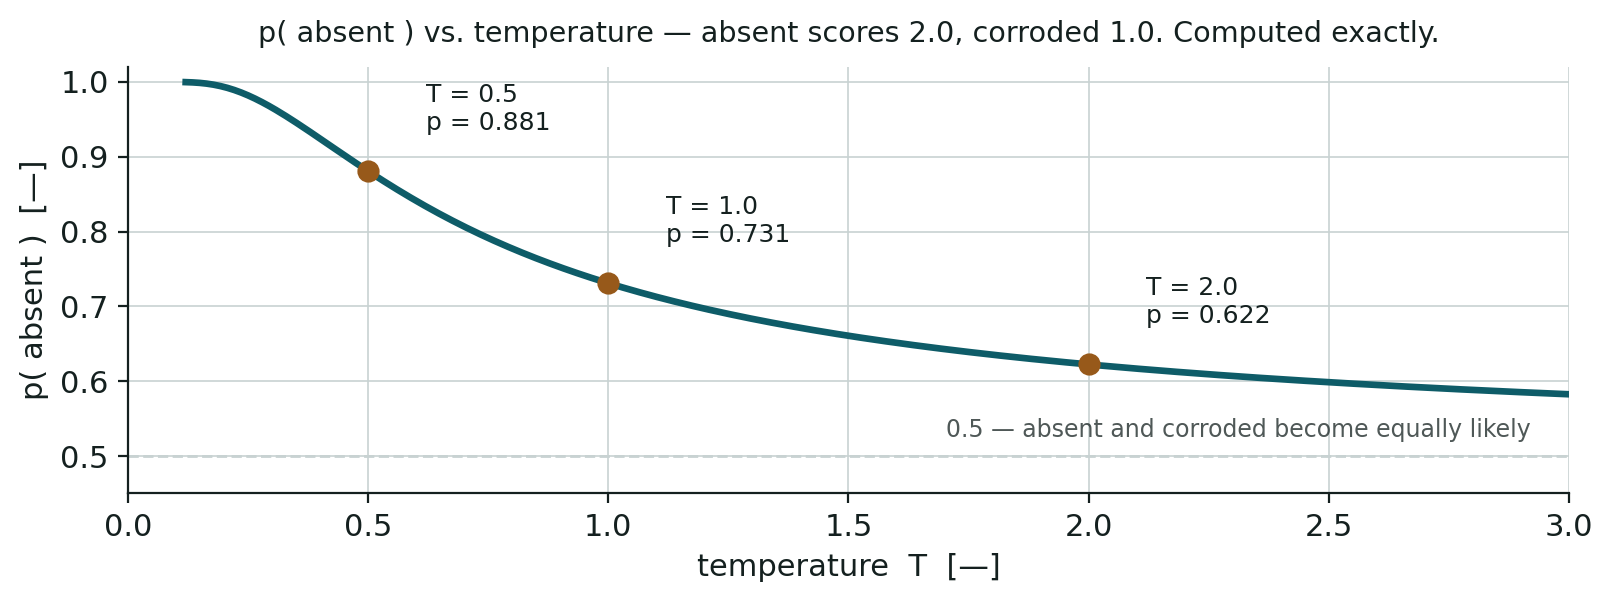
\includegraphics[height=30mm,width=\linewidth,keepaspectratio]{01-softmax-T}
    \end{column}
  \end{columns}
  \vspace{0.2em}
  \[ \mprob{p_i} = \frac{\exp(\mlogit{z_i}/{\color{uhred}\mathbf{T}})}{\sum_j \exp(\mlogit{z_j}/{\color{uhred}\mathbf{T}})} \]
  \vspace{-0.4em}
  {\small \kw{Low T} sharpens until one token takes almost everything; \kw{high T} spreads the
   \prob{probability} out. \kw{T} is a setting, not something the model computes.}
  \provenance{computed}
\end{frame}
\note{%
Temperature is a setting on the sampler, applied after the network has finished. It changes nothing
inside the network and nothing about training.\\[0.3em]
Watch the tail: at high temperature "blue" becomes reachable. That is the slide's second job ---
showing that the distribution covers every token in the vocabulary, not four.}

% ---------------------------------------------------------------- 19   (was 20)
\begin{frame}{Each token is appended and everything reruns}
  \begin{center}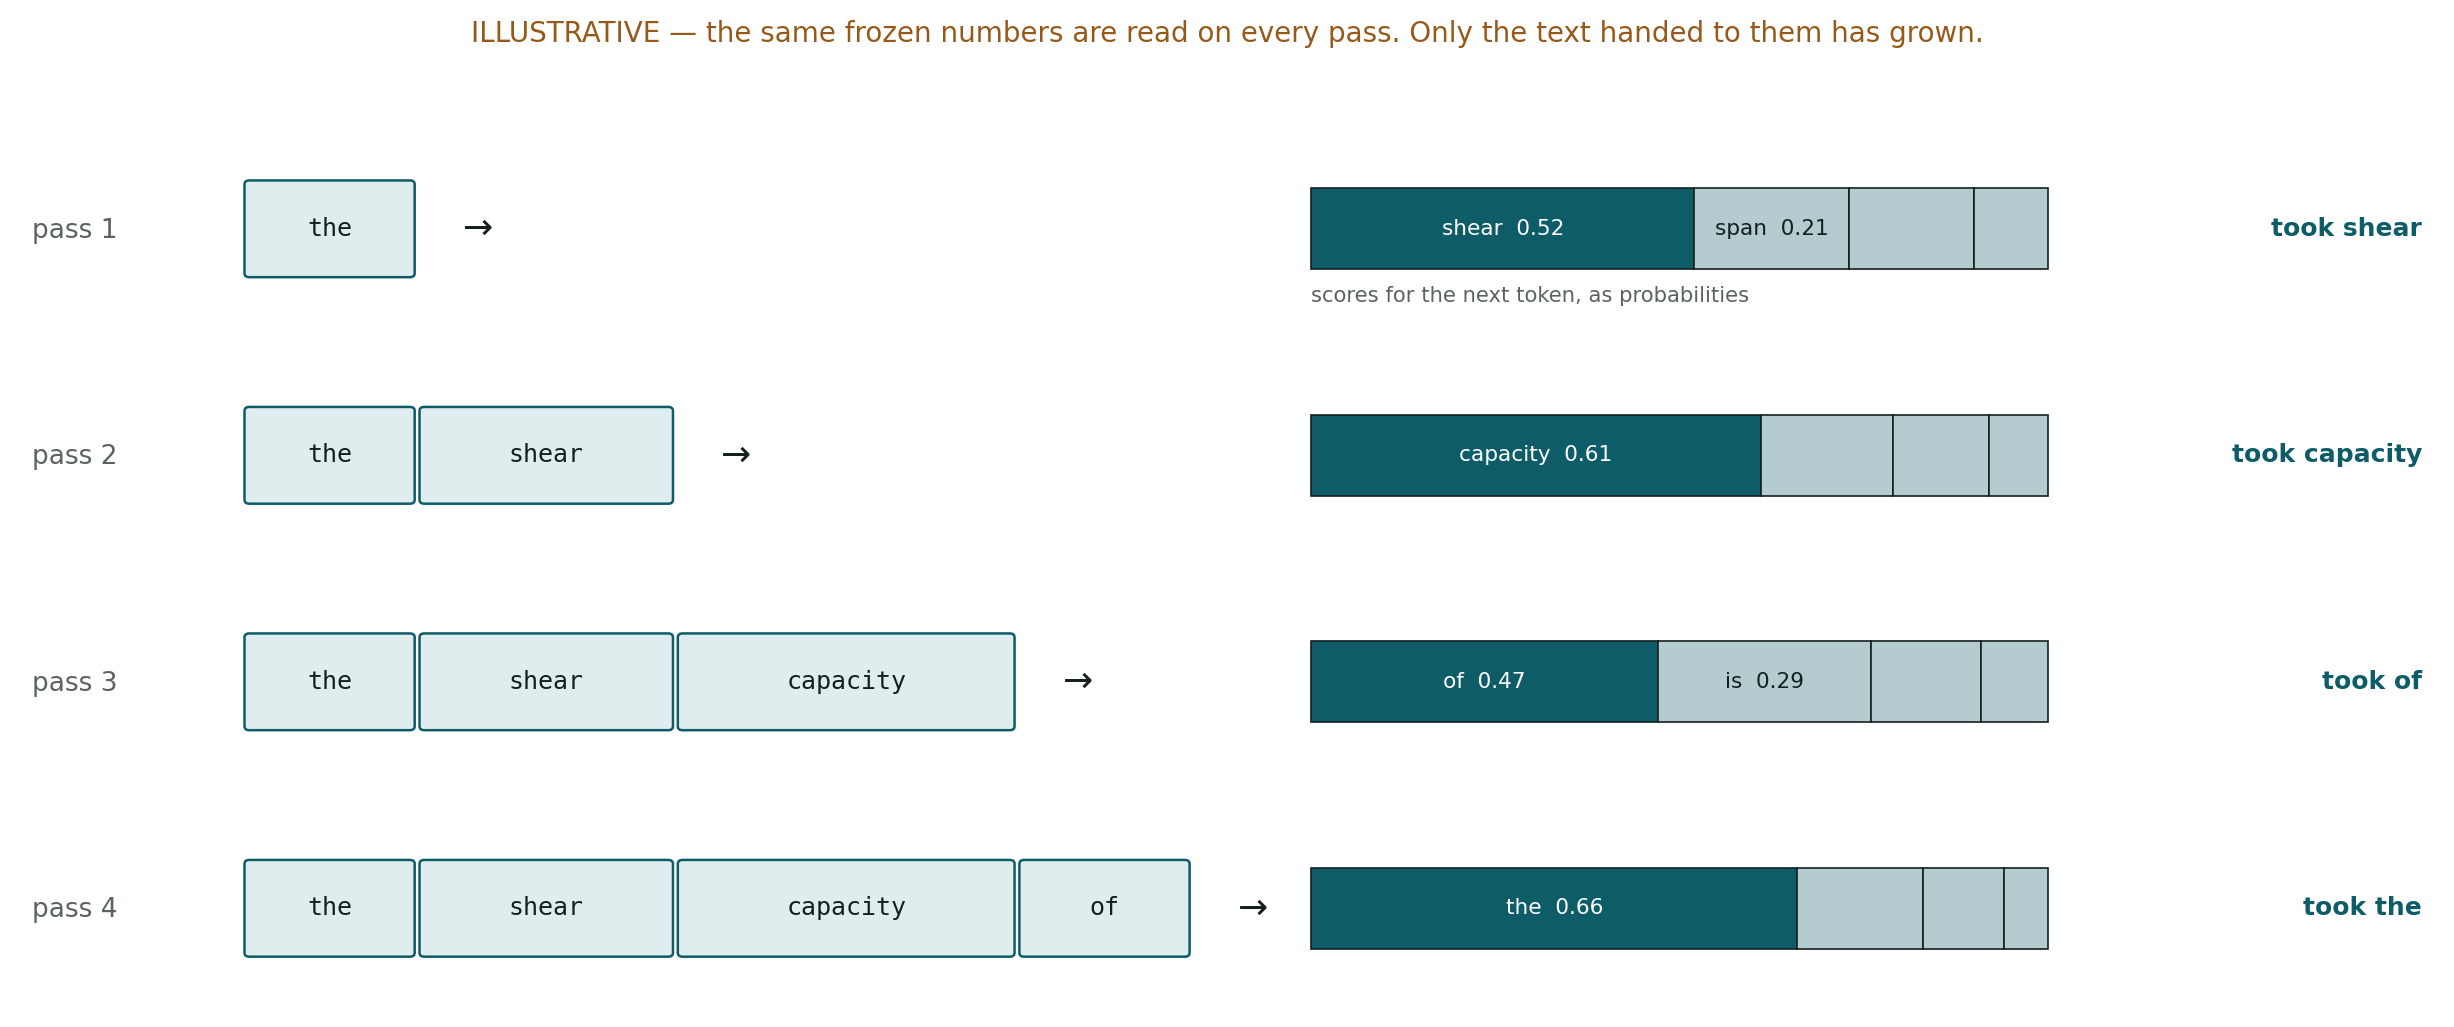
\includegraphics[height=40mm,width=\linewidth,keepaspectratio]{01-loop}\end{center}
  \animatable{A7}{1600 $\times$ 450 px}
  {\small The \param{parameters} are unchanged on
   every one of them.}
  \provenance{schematic}
\end{frame}
\note{%
Closes the loop the pipeline diagram opened, and explains the piece-at-a-time observation from
slide 2.\\[0.3em]
Every pass costs the same arithmetic, which is why output length and price track each other ---
Chapter 7 derives it and Chapter 13 bills it.\\[0.3em]
Generation cannot be parallelised across positions, because pass four needs the token pass three
produced. Training can be, which is why training a model is fast relative to the text it reads and
generation is not.}

% ---------------------------------------------------------------- 20   (was 11)
\begin{frame}{Everything given sits in the context window}
  \begin{center}
  \scalebox{0.58}{\begin{tikzpicture}[node distance=4mm]
    \node[uhbox]                       (a) {your prompt};
    \node[uhbox, below=of a]           (b) {files you pasted};
    \node[uhbox, below=of b]           (c) {the conversation\\so far};
    \node[uhbox, below=of c]           (d) {standing\\instructions};
    \node[uhbox, below=of d]           (e) {what a tool\\returned};
    \node[uhhi, right=16mm of b, yshift=-6mm, text width=30mm, minimum height=26mm]
                                       (w) {\textbf{the context window}\\[0.4em]a fixed maximum,\\counted in tokens};
    \node[uhbox, right=10mm of w]      (n) {the network};
    \node[uhghost, below=10mm of n]    (x) {everything else\\you ever wrote};
    \draw[uhar] (a)-|(w); \draw[uhar] (b)--(w); \draw[uhar] (c)-|(w); \draw[uhar] (d)-|(w);
    \draw[uhar] (e)-|(w);
    \draw[uhar] (w)--(n);
    \draw[uhardot] (x)-- node[right,font=\scriptsize\itshape,pos=0.4]{not supplied} (n);
  \end{tikzpicture}}
  \end{center}
  {\small Re-read in full every time the network runs. \kw{Standing instructions} are placed in the
   window at the start of every session. A \kw{tool} is a program run alongside the network, and its
   result is written into the window as tokens.}
  \citesource{anthropic-code-exec}
\end{frame}
\note{%
Box zero of the diagram, and it belongs here rather than at the end: the window is what the
model is handed, so it comes with the input stage.\\[0.3em]
The window is neither storage nor a database. It is an input buffer, and its contents are supplied
fresh on every pass.\\[0.3em]
Do not state a maximum size. Window sizes are per-model and per-plan, they change, and none is
cited here.\\[0.3em]
If asked how a conversation carries over: the application re-sends the whole conversation on every
turn. The network remembers nothing between turns; something outside it re-supplies the history.}

% ---------------------------------------------------------------- 21   (was 23)
\begin{frame}{The session ends and the window goes}
  \begin{center}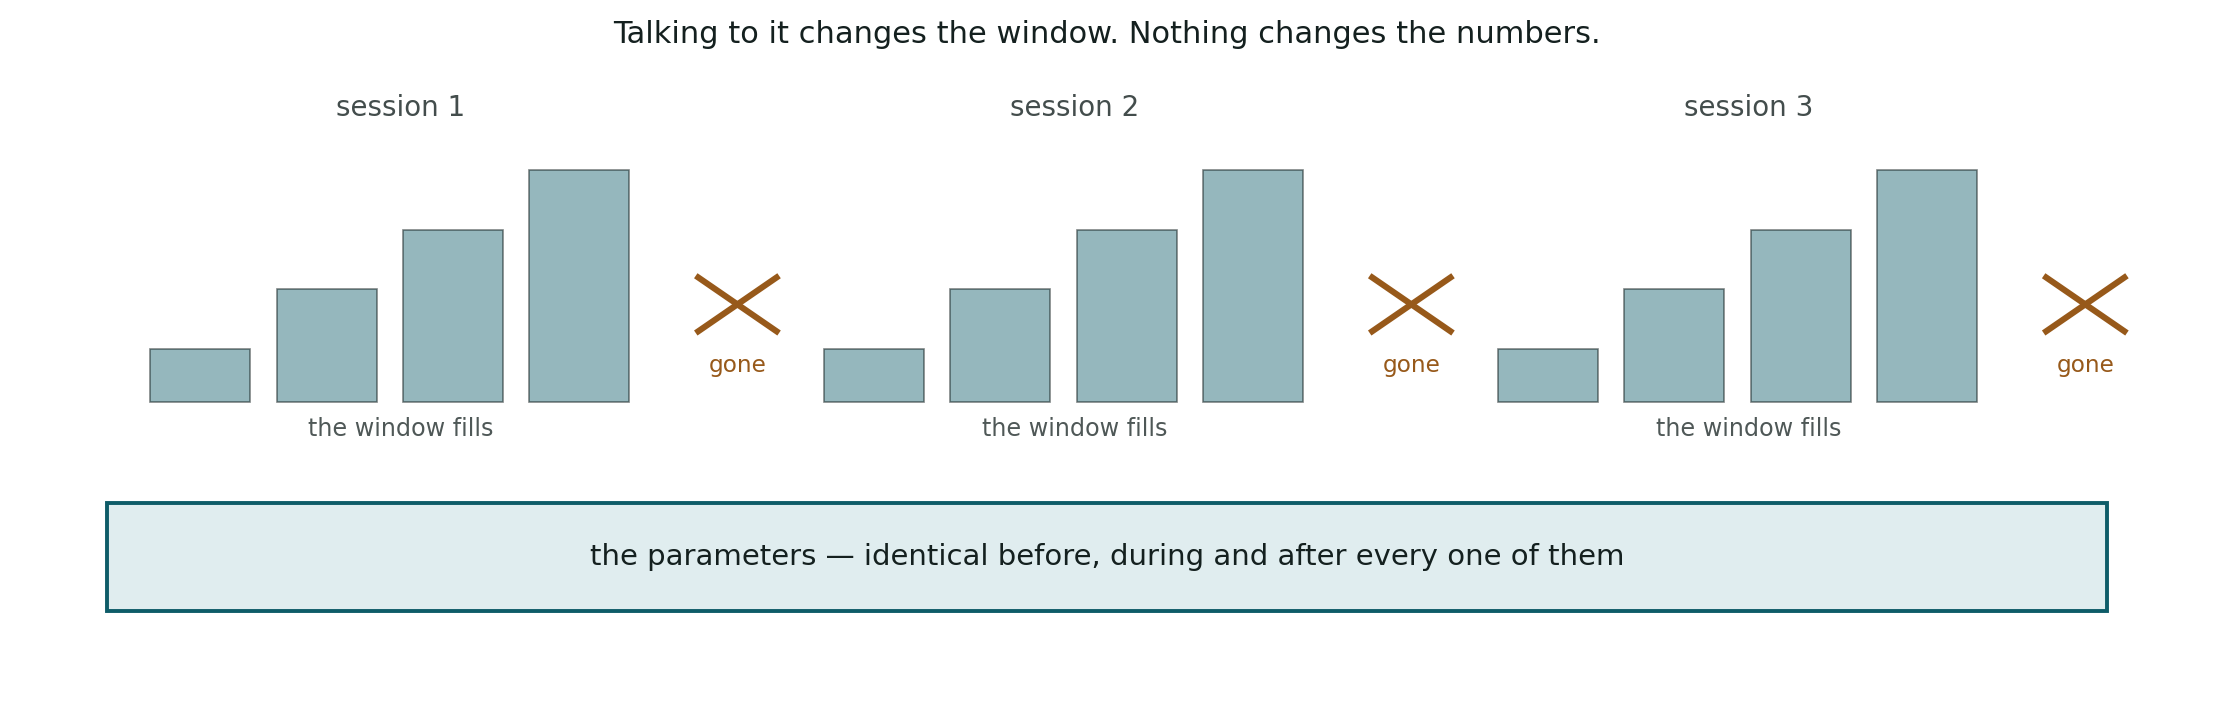
\includegraphics[height=33mm,width=\linewidth,keepaspectratio]{01-persistence}\end{center}
  \begin{columns}[t]
    \begin{column}{0.46\linewidth}\centering
      \kw{The network keeps nothing}\\[0.2em]{\small nothing you sent changed it}
    \end{column}
    \begin{column}{0.46\linewidth}\centering
      \kw{Unchanged}\\[0.2em]{\small the \param{parameters}, in every session}
    \end{column}
  \end{columns}
  \provenance{definition}
\end{frame}
\note{%
Talking to it teaches it nothing. Anything that looks like memory is a file being read back into
the window at the start of the next session, and Chapter 10 is where they write that file.\\[0.3em]
Caveat: providers may retain transcripts for their own purposes. That is a data-governance question
rather than a memory one, and Chapter 18 handles it.}

% ---------------------------------------------------------------- 22   (new)
\begin{frame}{Your brain divides the work into parts}
  \begin{center}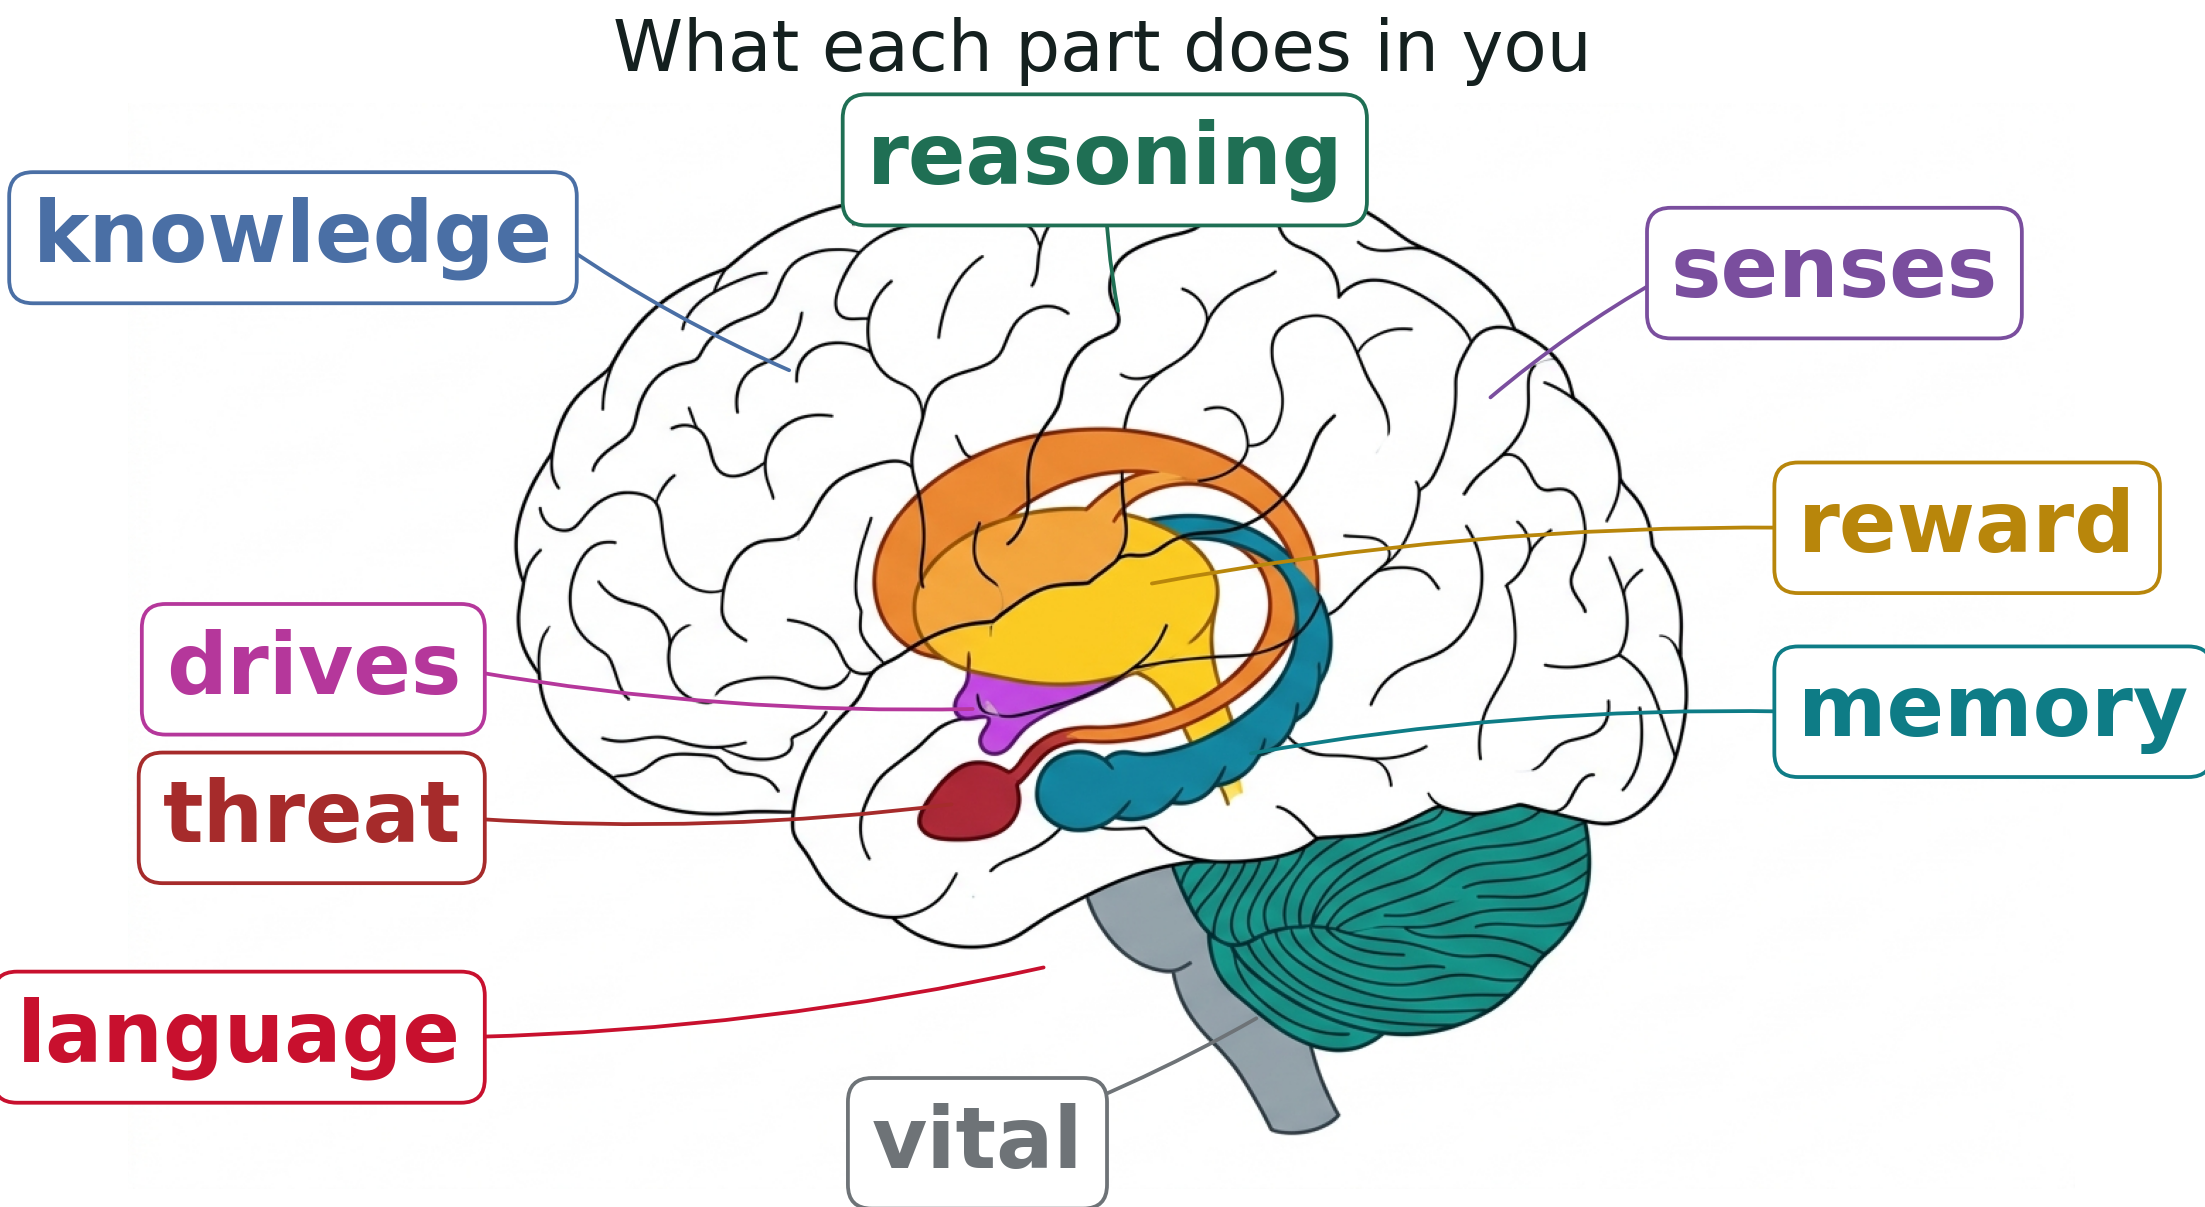
\includegraphics[height=46mm,width=\linewidth,keepaspectratio]{01-brain-human}\end{center}
  \provenance{schematic}
\end{frame}
\note{%
Deliver this orally. The slide carries one word per region on purpose.\\[0.3em]
Walk the nine and say what each does, briefly: the brainstem keeps you alive without being asked;
the basal ganglia and their dopamine signal are the reinforcement system, which is where habits and
rewards are learned; the hypothalamus holds the set points, so hunger and temperature are drives
you did not choose; the amygdala is fast, coarse threat detection that fires before you have
deliberated; the hippocampus holds recent experience and writes it into cortex; the cortex is where
consolidated knowledge sits; the fronto-parietal network does effortful reasoning; the language
network produces and understands language; sensory cortex turns light and pressure into
features.\\[0.3em]
The point of the frame is the picture, not the words. Every region is a separable part that can be
damaged on its own. Say that explicitly, because the next frame turns on it.\\[0.3em]
This is a left lateral view, which is the correct side: the language network is left-lateralised.\\[0.3em]
The illustration was generated; every label was placed by hand against anatomical sources. Regions
are shown schematically and boundaries are approximate. Do not defend the exact outlines.}

% ---------------------------------------------------------------- 23   (new)
\begin{frame}{One set of weights does every job}
  \begin{center}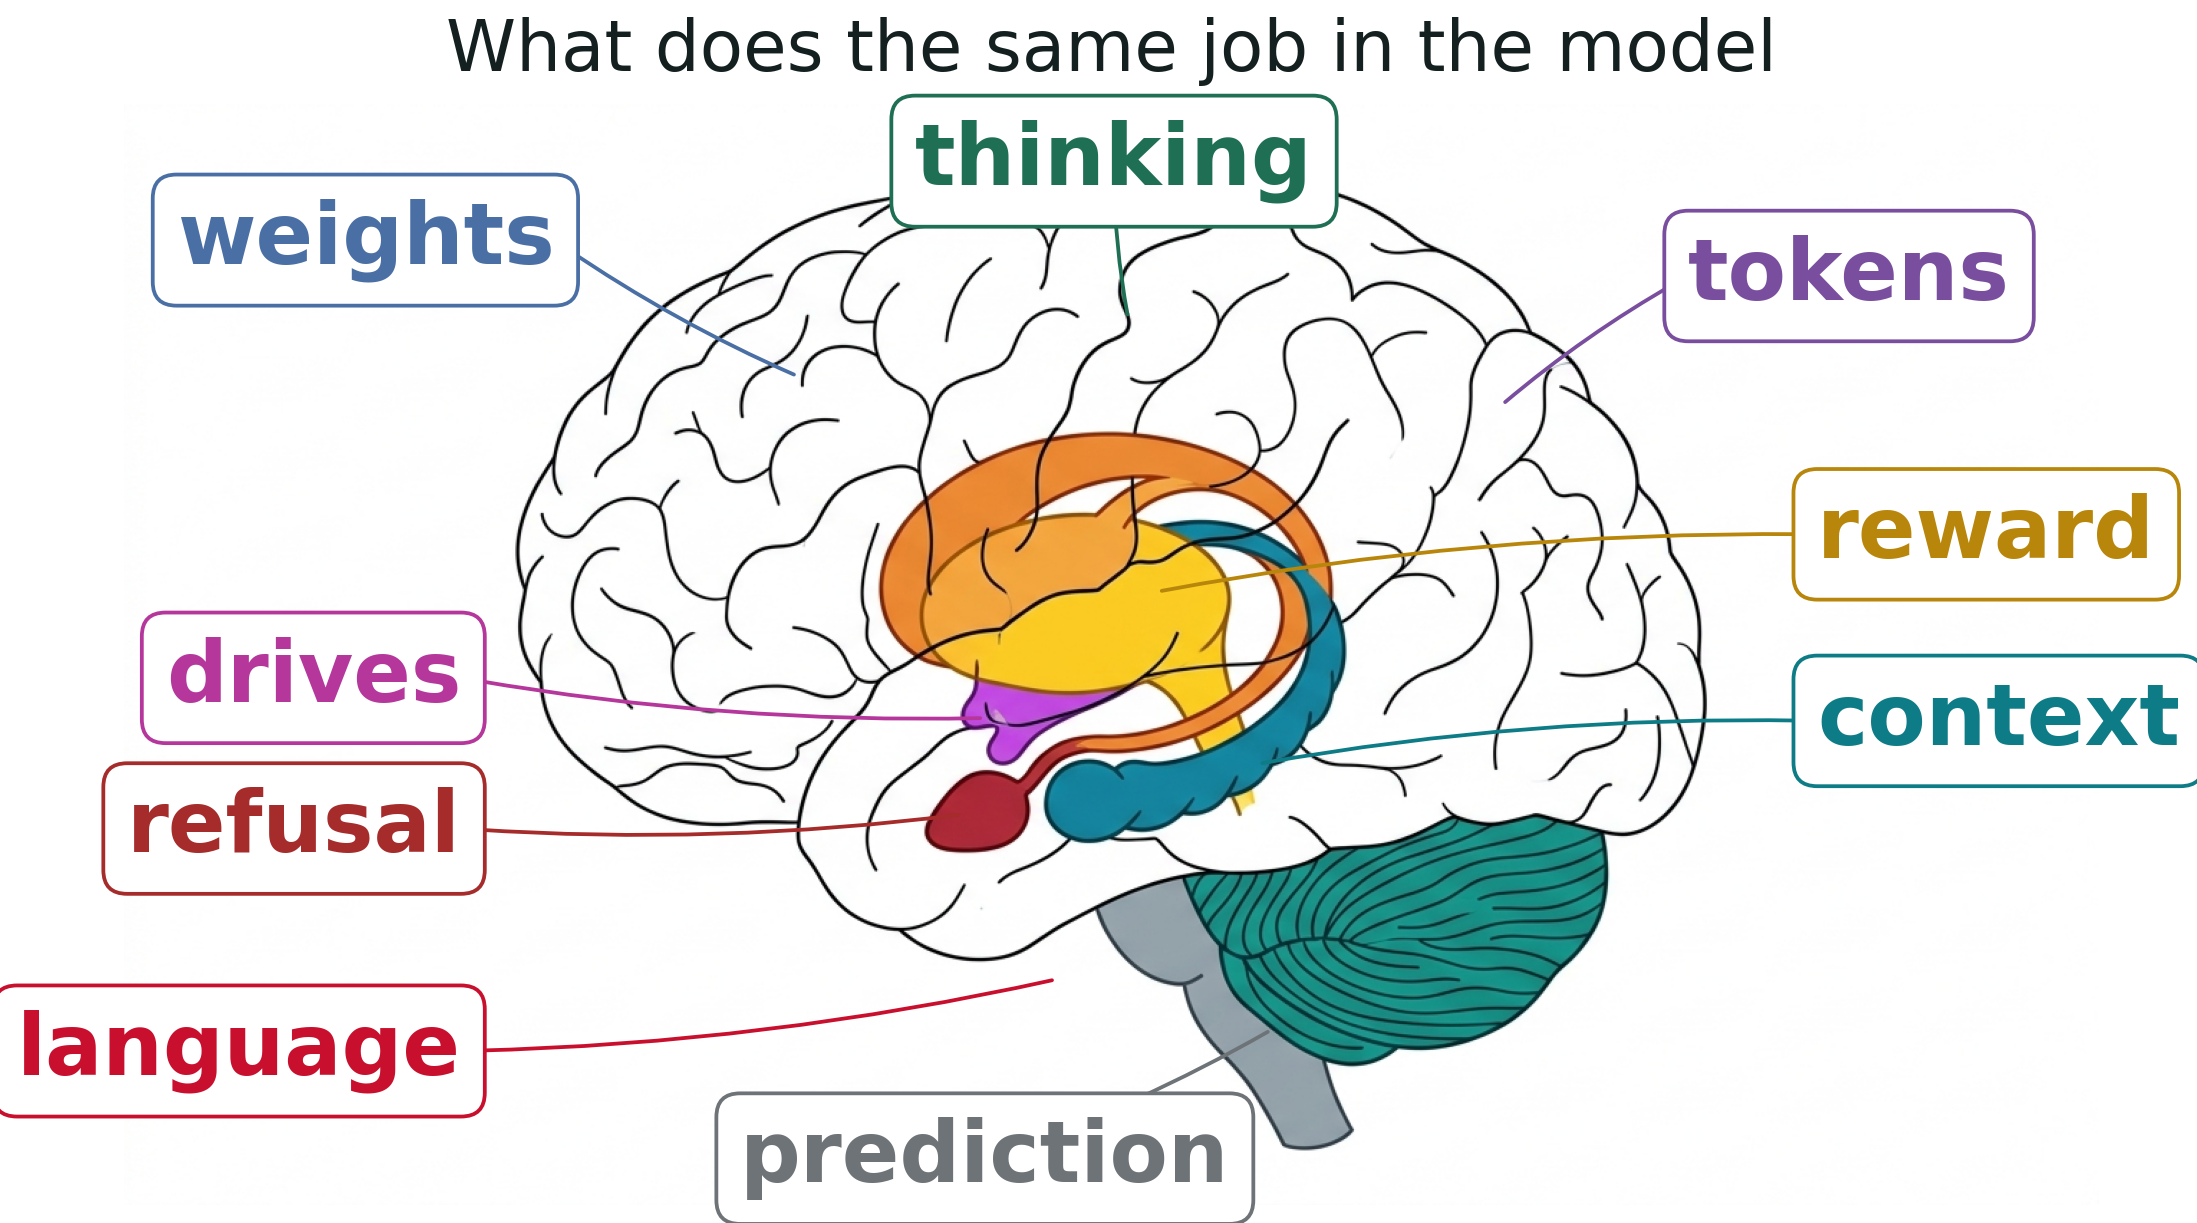
\includegraphics[height=38mm,width=\linewidth,keepaspectratio]{01-brain-model}\end{center}
  \vspace{-0.2em}
  {\small\textbf{Language and thought are separable systems in people, a double dissociation, and
   one set of weights in the model.}}
  \citesource{fedorenko2024}
\end{frame}
\note{%
Same picture, same colours, the words swapped. Let the room notice before you say anything.\\[0.3em]
Then give the pairs and, for each, where it breaks. Next-token prediction is the base drive, the
thing that never stops, and everything else was installed on top of it. The reward model and RLHF
are the reinforcement layer, and the maths is genuinely the same idea as the dopamine prediction
error, but yours runs for life and this ran once and stopped. The trained dispositions are the
drives, and here is the sharp difference: a paragraph of system prompt can change the model's
drives, and nothing anybody says will talk you out of being hungry. Refusal behaves like threat
detection, fast and coarse and fired by surface features, which is exactly why a harmless request
sometimes gets refused. The context window is the holding part of memory with the writing part
missing, which is why Chapter 10 exists. The weights are the consolidated knowledge, frozen where
yours keeps updating. Thinking is effortful reasoning, except that it is a dial someone outside can
turn, and it spends tokens rather than building capacity.\\[0.3em]
On effort, if asked: it controls tokens. Thinking is the model generating reasoning text before the
answer, through the same network, so more effort means more passes, and time and cost follow from
that. Thinking and the answer share one output budget.\\[0.3em]
The closing line is the payoff and it is sourced. In people, language and thought can be damaged
independently, which is what a double dissociation means. In the model there is nothing to
dissociate. That is not a defect: it is why one model moves between summarising, coding and arguing
without switching systems. It is also why fluency tells you nothing about whether the content is
right, because there is no second system whose health the fluency could be reporting.\\[0.3em]
That is the argument for everything the rest of the course does about verification.}

% ---------------------------------------------------------------- 24   (was 24)
\begin{frame}{What we covered, and what is still open}
  \begin{columns}[t]
    \begin{column}{0.49\linewidth}
      {\usebeamercolor[fg]{frametitle}\bfseries What we covered}\\[0.5em]
      {\footnotesize
      \begin{itemize}\itemsep0.25em
        \item A model is a list of \param{numbers} and a program that reads them
        \item Training fixed those numbers and stopped
        \item What it minimised was surprise, so the output is a \prob{distribution}
        \item Text is cut into \tokid{tokens} from a fixed list
        \item Every pass scores every token, then draws one
        \item It sees only the context window, and discards it
      \end{itemize}}
    \end{column}
    \begin{column}{0.49\linewidth}
      {\usebeamercolor[fg]{frametitle}\bfseries What is still open}\\[0.5em]
      {\footnotesize
      \begin{itemize}\itemsep0.25em
        \item Nothing in scoring text makes a thing that answers a question, follows an
              instruction, or declines a request. What was added?
        \item Why does it agree with you so readily?
        \item If it is reliable where much has been written, how do you tell which regime you
              are in?
        \item How would you ever know a change to your prompt actually helped?
      \end{itemize}}
    \end{column}
  \end{columns}
  \provenance{derived}
\end{frame}
\note{%
The takeaway for anyone attending only this session, and what the reference card carries.\\[0.3em]
The open questions are the handoff. The first is Chapter 2, the second is Chapter 2, the third is
Chapter 5, the fourth is Chapter 4. Do not print the chapter numbers --- say them if asked.\\[0.3em]
Excluded from this chapter, if asked: how attention weights are computed, positional encoding,
multi-head attention, and the KV cache. The first three change no decision anyone here makes. The
KV cache is defined in Chapter 7, where it is priced.}

\end{document}
